% !TEX root = ../double_trouble_supp.tex

In this section we provide additional experimental evidence of the predictive performance on synthetic and real genomic data of our newly proposed BNP model as well as a number of preexisting competing (single population) methods.
Specifically, we consider the d3BP, i3BP (as defined in \cref{sec:d3BP,sec:i3BP}), as well as the Good-Toulmin (GT) estimator --- recently employed by \citet{chakraborty2019using} in the context of rare genomic variants discovery --- and the fourth order Jackknife estimator (4JK) \citet{gravel2014predicting}. We additionally consider a linear programming approach \citep[LP]{zou2016quantifying}, and the scaled process (SP) method by \citet{Camerlenghi2021}. In real data experiments we choose the best performing single population method and apply it in two different ways --- namely assuming both (i) that populations are independent and do not share variants and (ii) that samples are in fact obtained from a single population.

\subsection{Additional synthetic experiments}
\label{sec:misspecified}

Here we generate data from the i3BP and the d3BP to test the performance of our model under these types of misspecification (either no shared variants as in the i3BP, or no heterogeneity across populations as in the d3BP). 

For the i3BP, we generate data using a three parameter Indian buffet process, \citep{Broderick2012, Masoero2022}, assuming there are no shared variants across the two populations. For the d3BP, we generate variants from a single Indian buffet process and then randomly split individuals into two populations. 

In our plots, we use the \emph{relative residual} as a measure of accuracy. Namely, the signed difference between a method’s prediction and the observed value in the reserved follow-up data, normalized by the observed value.


\paragraph{Data from the i3BP}

For the i3BP, we consider two sets of values for the hyperparameters $(\alpha_1,c_1,\sigma_1,\alpha_2,c_2,\sigma_2)$: $(20,1,.6,20,1,.3)$, and   $(40,1,.1,40,1,.3)$ where $(\alpha_\popidx, c_\popidx, \sigma_\popidx)$ are the corresponding 3BP's mass, concentration and discount parameters in population $\popidx$. 

\begin{figure}[htp]
    \centering
    \includegraphics[width = 0.9\textwidth]{Ch2-double-trouble/Figs//i3BP_20fold.png}
    \includegraphics[width = 0.9\textwidth]{Ch2-double-trouble/Figs//i3BP_slow_20fold.png}
    \caption{Prediction when data is sampled from the i3BP. Each row represents a different simulated dataset, as described in Section 8.1. 
    \emph{Left}: The dashed black line shows the observed number of variants as a function of the number of samples. The samples appear in the following order: the pilot from population 1, the pilot from population 2, the follow-up from population 1, the follow-up from population 2. A vertical dashed gray line separates the two populations in the pilot and follow-up, respectively. The gray shading covers the pilot data. All curves agree exactly on the pilot data. In the follow-up region, we plot the mean (lines) and 1 standard deviation intervals (shaded regions) from the three methods: our proposed method (solid red), the dependent version of the single-population 3BP (dash-dot blue), and the independent version of the 3BP (dotted green).  
    \emph{Center and Right}: For each $\vecoccurrence$ with component values up to 10, we plot the relative residual for predictions from our method (right) and the dependent 3BP (center), average over folds. \revision{Note that the color scales in residual plot are different across datasets.} A square is gray when the observed value is strictly less than 2 in at least one fold or $\vecoccurrence = (0,0)$.  
    }
    \label{fig:i3BP}
\end{figure}

We show in \Cref{fig:i3BP} the ground truth rate of growth of number of variants as a function of the sample size, as well as the corresponding curves stemming from the predictions of all three models (i3BP, d3BP, our proposed multi population model). In this setting, our method seems to be roughly unbiased, much like the correctly specified i3BP model. \minorrevision{A slight overestimation exists at the end, which might be due to misspecification or misestimation of the rate of the second population during fitting.} However, our model does incur larger variance in the estimates, potentially due to the wrong assumption that all variants are eventually shared across populations. Meanwhile, as expected, the d3BP vastly underestimates the number of $\bm{k}$-tons, especially for \minorrevision{ $k_1=0, k_2>0$ or $k_1>0, k_2=0$ }as it assumes that all variants share the same frequencies in the two populations, \revision{an assumption that would lead to a low number of variants that exist in only one population but not the other}. We emphasize that the overestimation of singletons by the d3BP is not surprising \revision{($(1,0)$-tons and $(0,1)$-tons in \cref{fig:i3BP})} since singletons are more compatible with the assumption that all variants share the same frequencies, and the fact that they are discovered in one or the other population is simply due to chance. 

\paragraph{Data from the d3BP}

We sample data from the d3BP by fixing the hyperparameters at $(\alpha,c,\sigma)=(20,1,.5),(40,1,.1)$  respectively. 


\begin{figure}[htp]
    \centering
    \includegraphics[width = 0.9\textwidth]{Ch2-double-trouble/Figs//d3BP_20fold.png}
    \includegraphics[width = 0.9\textwidth]{Ch2-double-trouble/Figs//d3BP.1_20fold.png}
    \caption{Prediction when data is sampled from the d3BP. Each row represents a different simulated dataset, as described in Section 8.1. \emph{Left}: The dashed black line shows the observed number of variants as a function of the sample number. The samples appear in the following order: the pilot from population 1, the pilot from population 2, the follow-up from population 1, the follow-up from population 2. A vertical dashed gray line separates the two populations in the pilot and follow-up, respectively. The gray shading covers the pilot data. All curves agree exactly on the pilot data. In the follow-up region, we plot mean (lines) and 1 standard deviation intervals (shaded regions) from three methods: our proposed method (solid red), the dependent version of the single-population 3BP (dash-dot blue), and the independent version of the 3BP (dotted green).  \emph{Center and Right}: For each $\vecoccurrence$ with component values up to 10, we plot the relative residual for predictions from our method (right) and the dependent 3BP (center), average over folds. \revision{Note that the color scales in residual plot are different across datasets.} A square is gray when the observed value is strictly less than 2 in at least one fold or $\vecoccurrence = (0,0)$. }
    \label{fig:d3BP}
\end{figure}


We show in \Cref{fig:d3BP} the ground truth rate of growth of number of variants as a function of the sample size, as well as the corresponding curves stemming from the predictions of all three models (i3BP, d3BP, our proposed multi population model). The hyperparameters were specified in such a way that the data has a relatively large number of shared variants. Thus, the i3BP method  --- which assumes no sharing --- incurs a significant level of double counting \revision{(a more extreme version of this can be seen in \cref{sec:slow_growth})}. Our proposed method also struggles when the power law rate is small with perfect correlation. This is understandable since our method restricts the form of correlation and does not put mass perfectly along the diagonal especially for relatively common variants (Figure 1, third panel). Specifically when the power-law rate is low, the total number of variants are not dominated by extremely rare singletons and our method's mispecification for relatively common variants could struggle. \revision{When the power-law rate is small under the d3BP, there are not many variants and a large portion of them should be relatively common. 
Recall that we fit our model's hyperparameter using variants with low frequencies in the training set. 
And under d3BP with a small rate, these variants are sparse and with limited amount of data, it is hard for our model to approximate d3BP given the flexibility but misspecification of our model. }



\subsection{Performance of single-population models on real data}

\label{sec:single_pop_methods}

We start by providing additional results on the performance of competing models when predicting the total number of genomic variance on real data in the presence of a single population.
For these comparisons, we tested fourth-order jackknife \citep[4JK,]{gravel2014predicting}, the Good-Toulmin estimator \citep[GT,]{Orlitsky2016,chakraborty2019using}, linear programming \citep[LP]{zou2016quantifying}, the 3BP approach of \citet{Masoero2022} \internal{and the scaled process (SP)} method by \citet{Camerlenghi2021}.
We consider both data coming from the GnomAD dataset \citep{karczewski2020mutational}, as well as cancer data from the cancer genome atlas (TCGA) and the MSK-impact dataset \citep{cheng2015memorial}.
We observe that on the cancer datasets, the 3BP and the SP perform very similarly. \internal{We compare our method to 3BP because it has the smallest root mean square error (RMSE) in predicted growth curve across folds (MSK-impact: 3BP: 2083.2 vs SP 2123.6 in breast cancer and 3BP 742.1 vs SP 789.2 in lung cancer; TCGA: 604.6 vs 632.8 in breast cancer and 1350.8 vs 1407.3 in lung cancer).} On the cancer data, these BNP approaches outperform the \internal{jackknife, GT, and linear programming methods.} The jackknife performs better than other competing methods in GnomAD datasets \internal{in RMSE}. 

We provide a summary of our findings with results on \internal{two largest cancer types, namely the breast and lung cancers} in \cref{fig:brca_luad_singlepop} and for a few subpopulations in the GnomAD dataset in \cref{fig:seu_bgr_singlepop}. 

\begin{figure}[H]
    \centering
    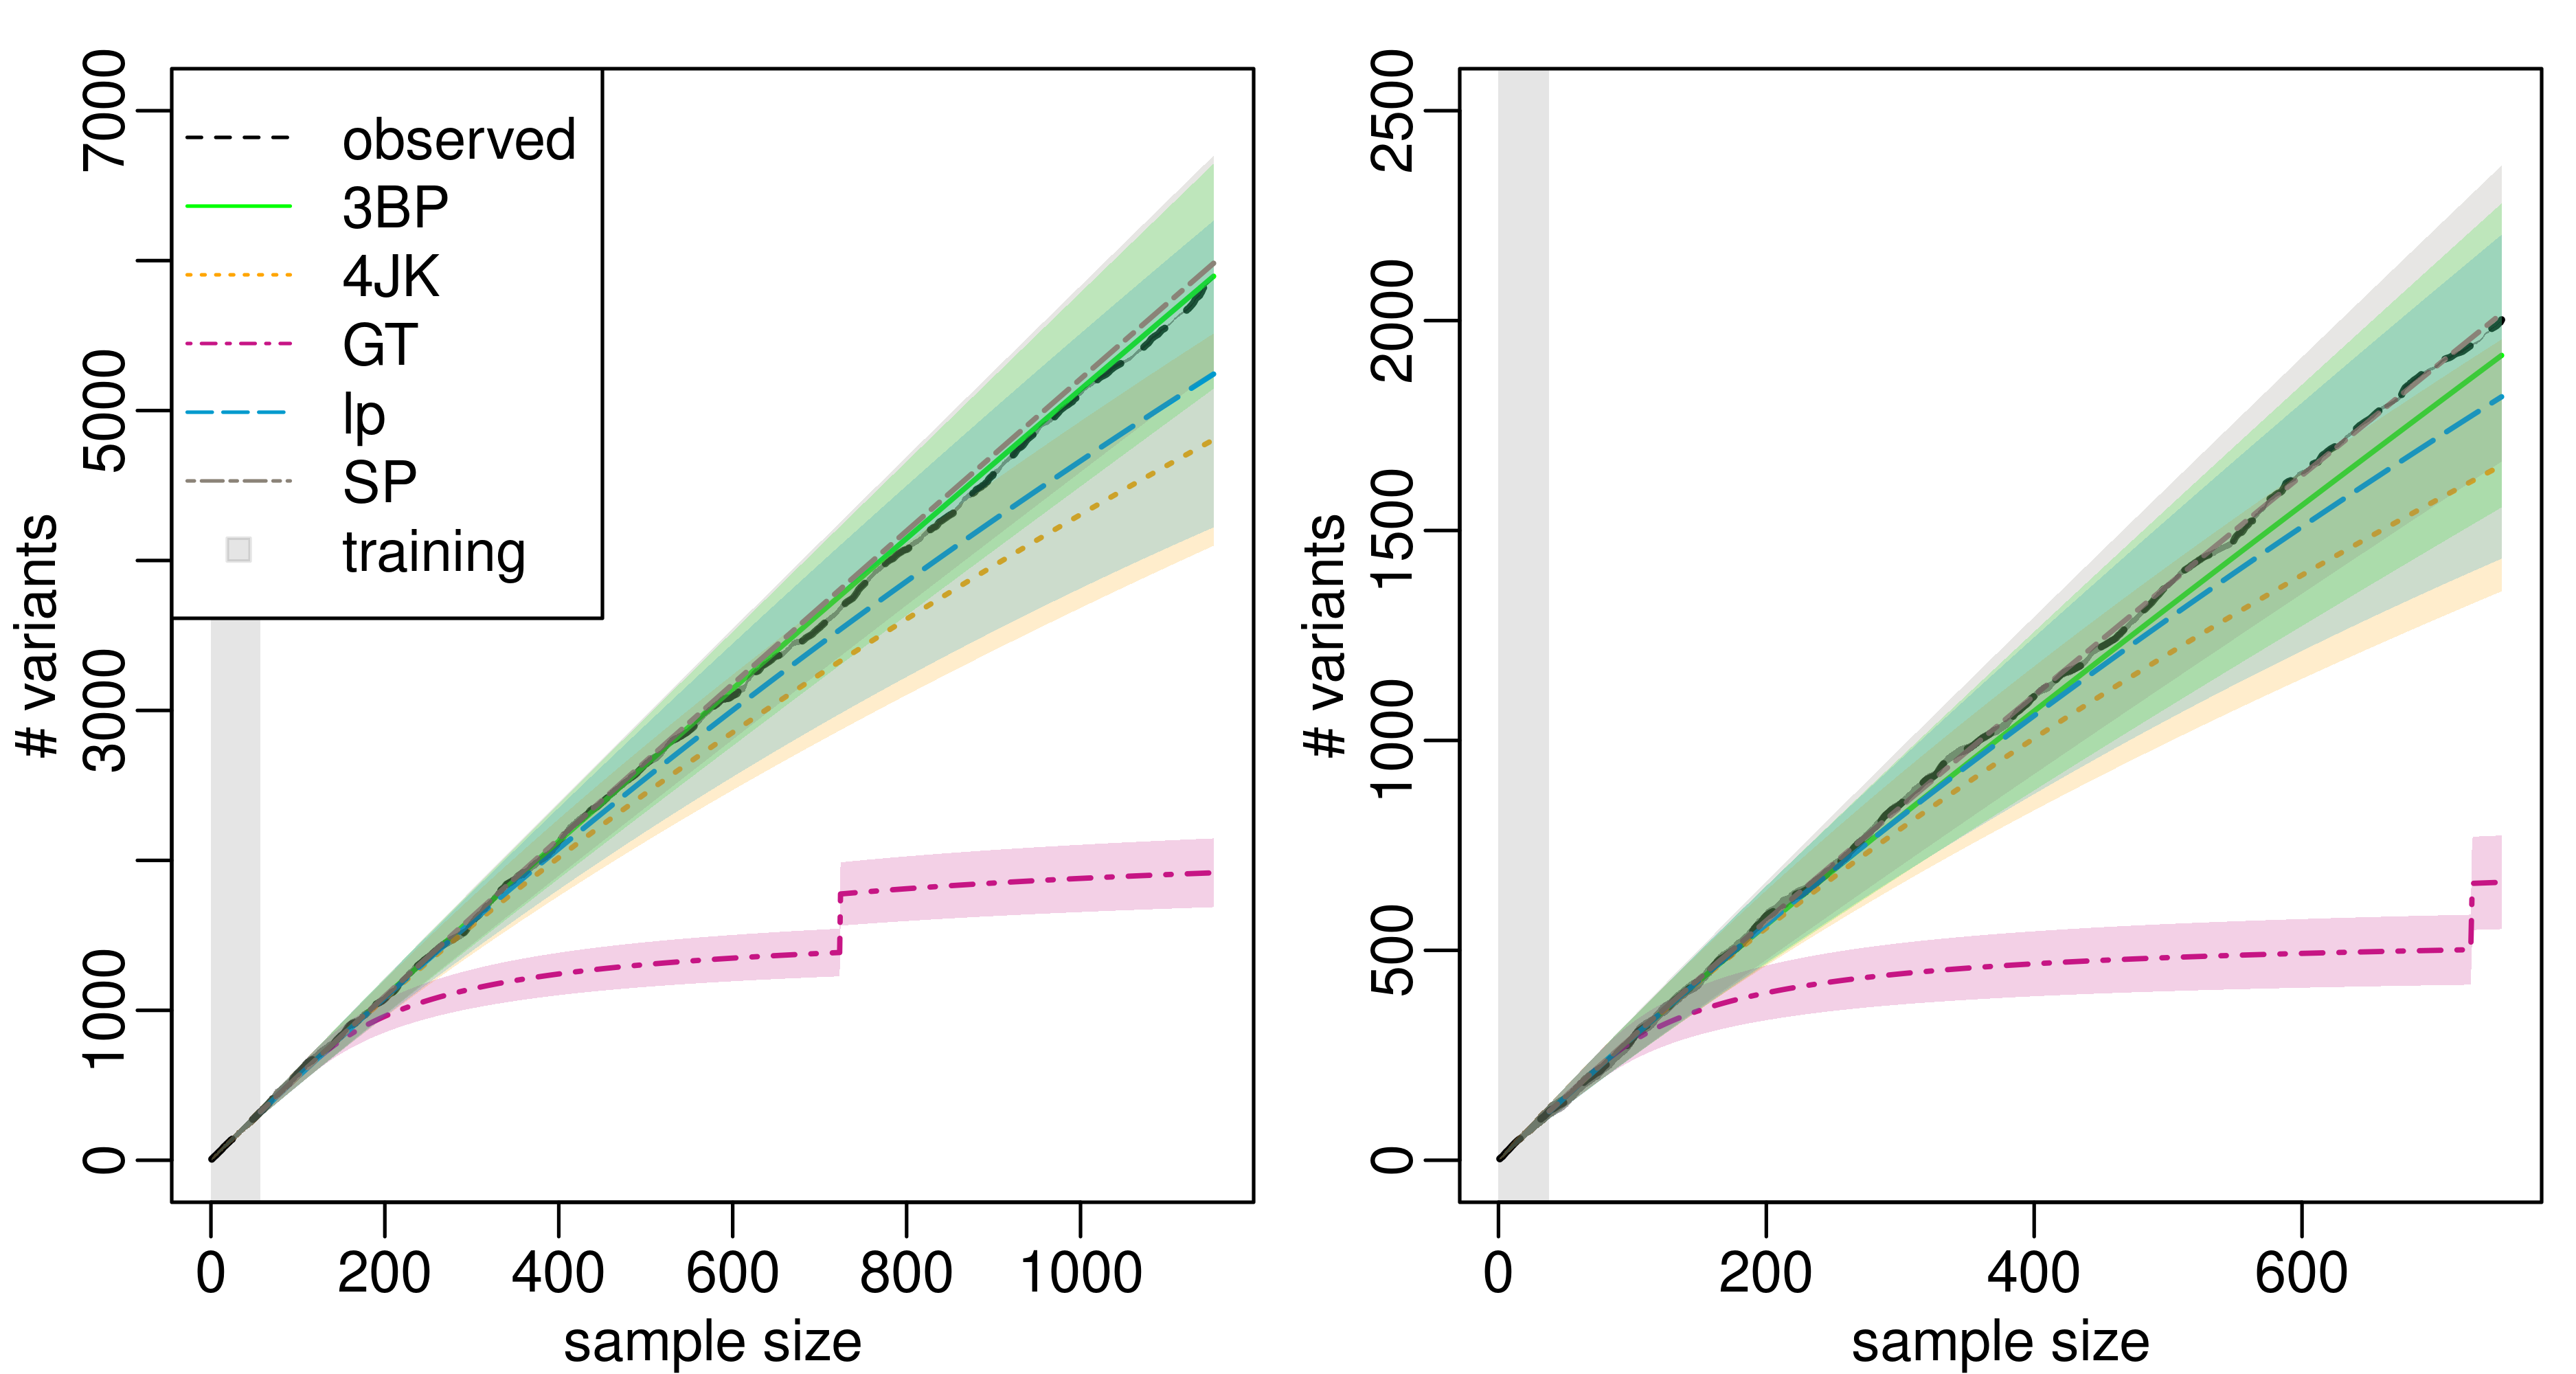
\includegraphics[width = 0.6\textwidth]{Ch2-double-trouble/Figs//BIDC_LA2_20fold_one_pop.png}
    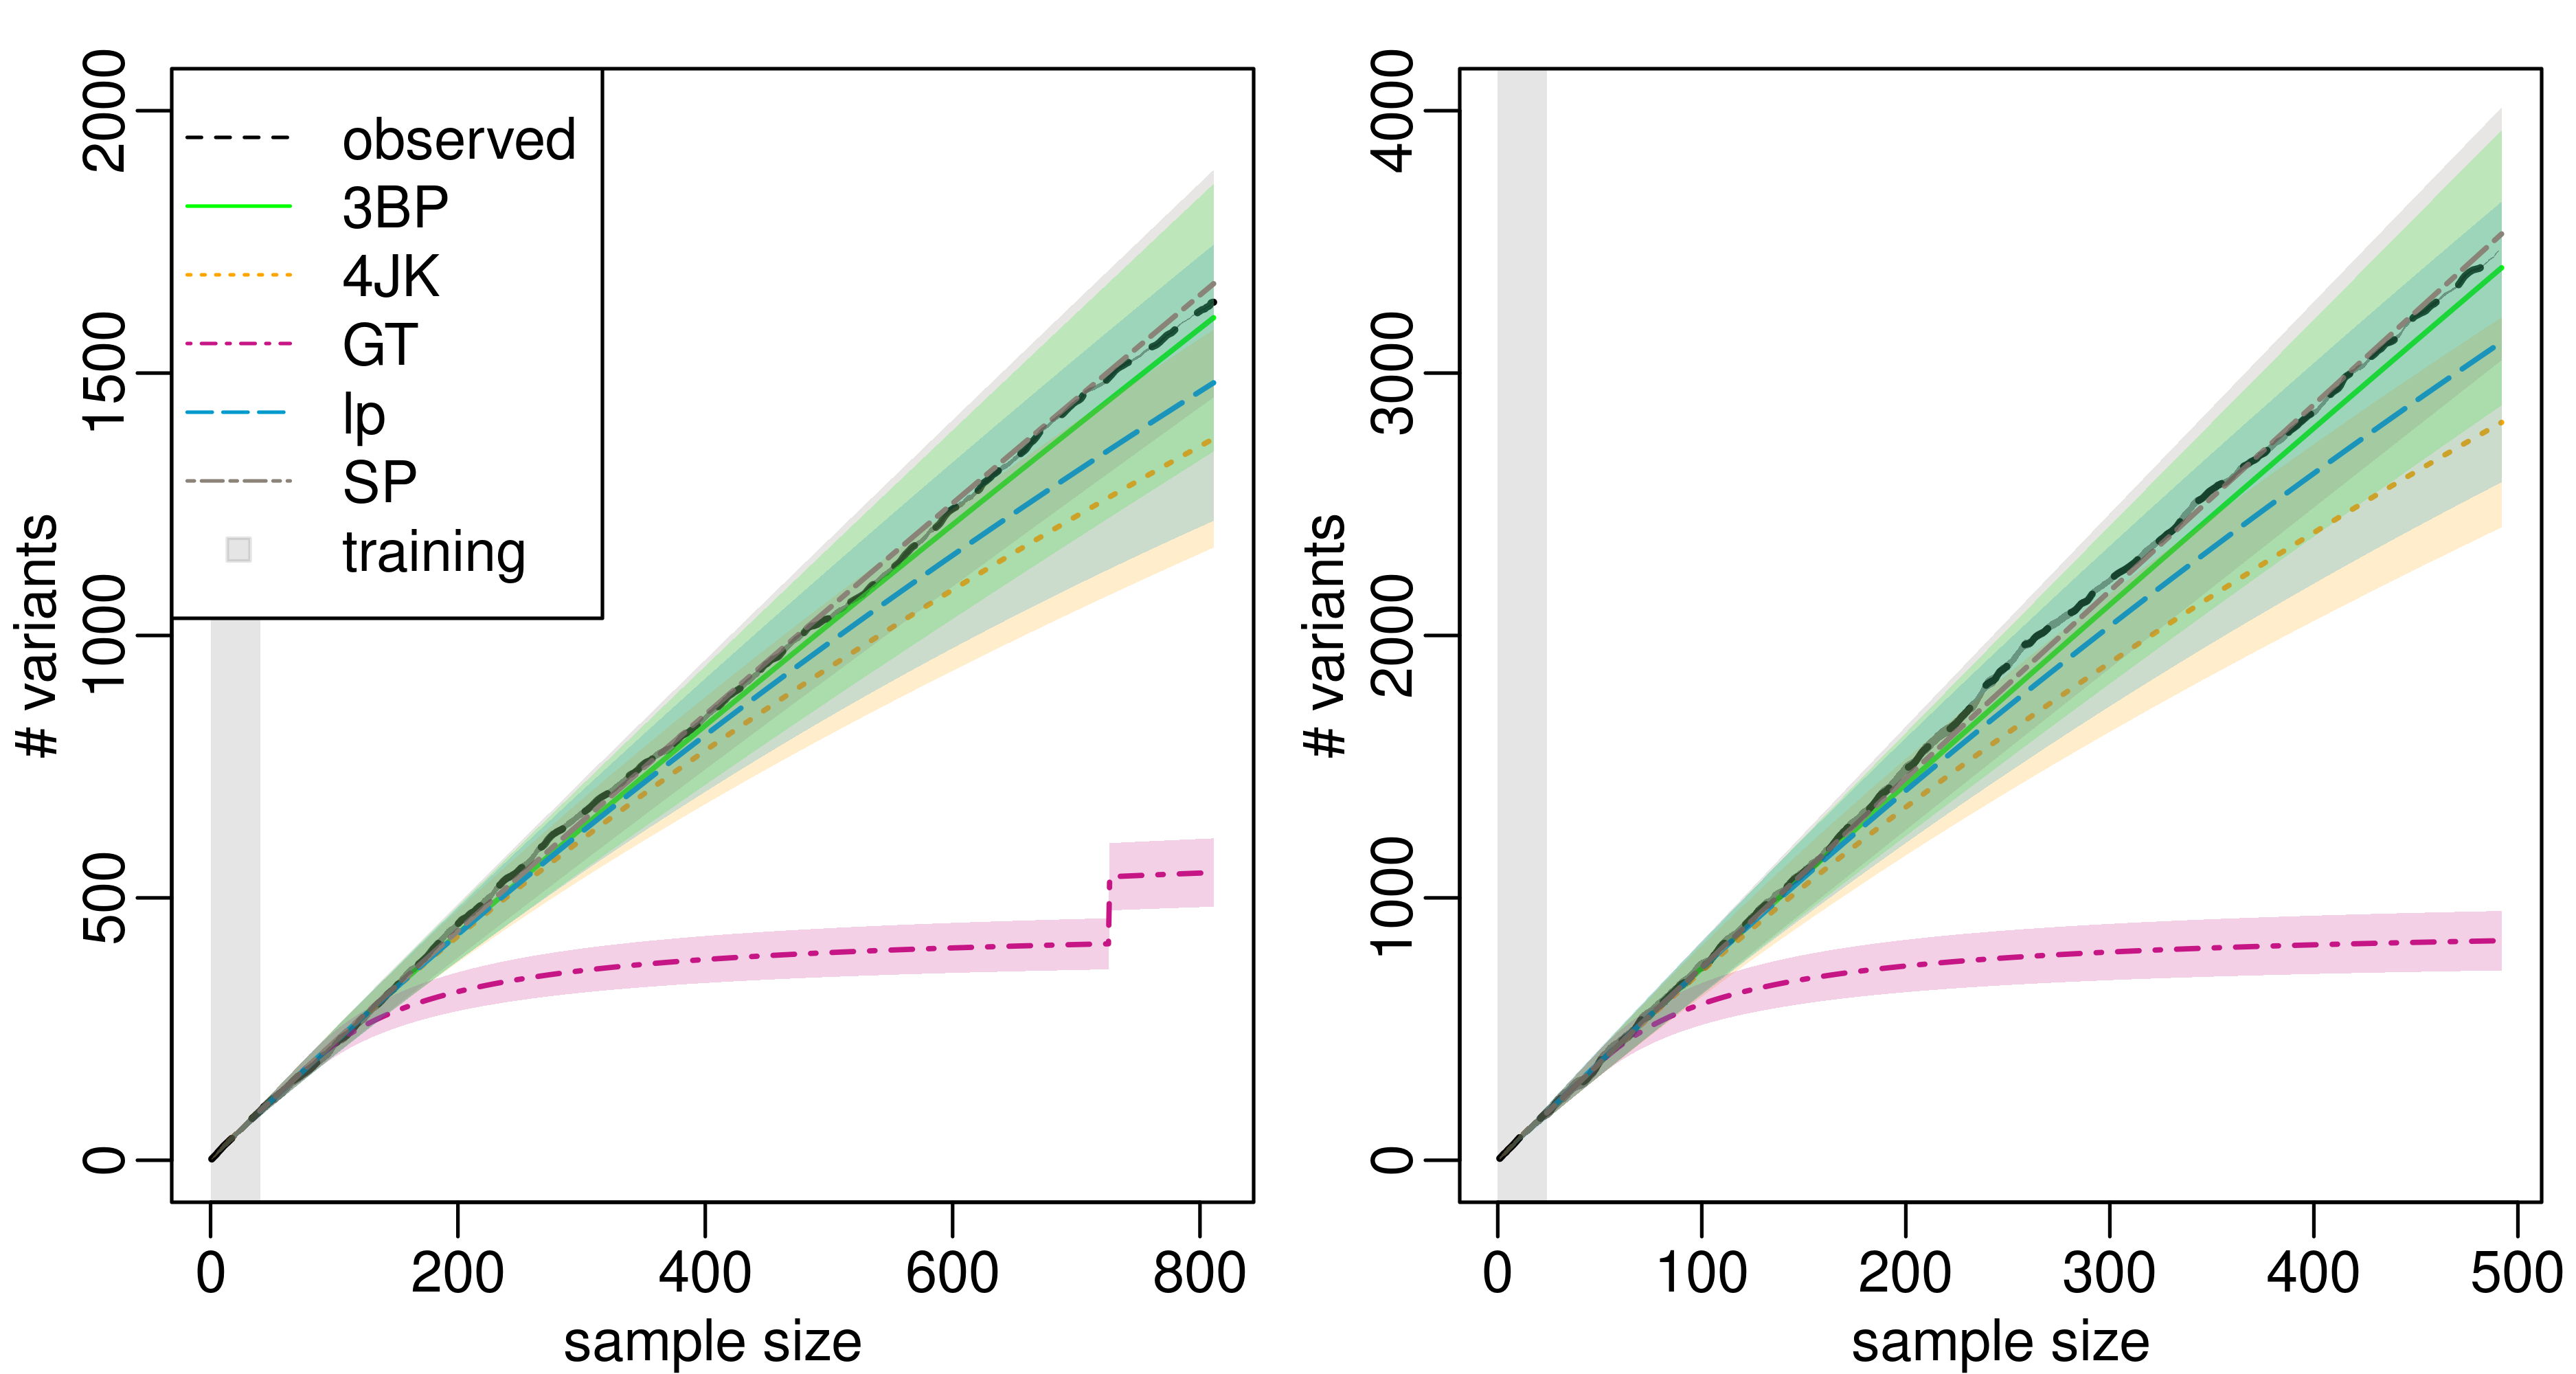
\includegraphics[width = 0.6\textwidth]{Ch2-double-trouble/Figs//BRCA_LUAD_20fold_one_pop.png}
    \caption{Prediction for the variant counts in, breast (left column) and lung cancer (right column) in the MSK-IMPACT dataset (first row) and TCGA dataset (second row) respectively. The dashed black line shows the observed number of variants as a function of the sample number. The samples appear in the following order: the pilot and then followup. The gray shading covers the
    pilot data. All curves agree exactly on the pilot data. In the follow-up region we plot mean (lines) and 1 standard deviation interval (shaded area) from five candidate single population models: 3BP (solid green), fourth order jackknife (dotted orange), GT (purple dot-line), linear programming (dashed cyan) and scaled process (dot dashed gray). The 3BP method outperforms or \revision{is comparable to} alternatives in this dataset. }
%    \label{fig:bidc_la2_singlepop}
    \label{fig:brca_luad_singlepop}
\end{figure}

\begin{figure}[H]
    \centering
    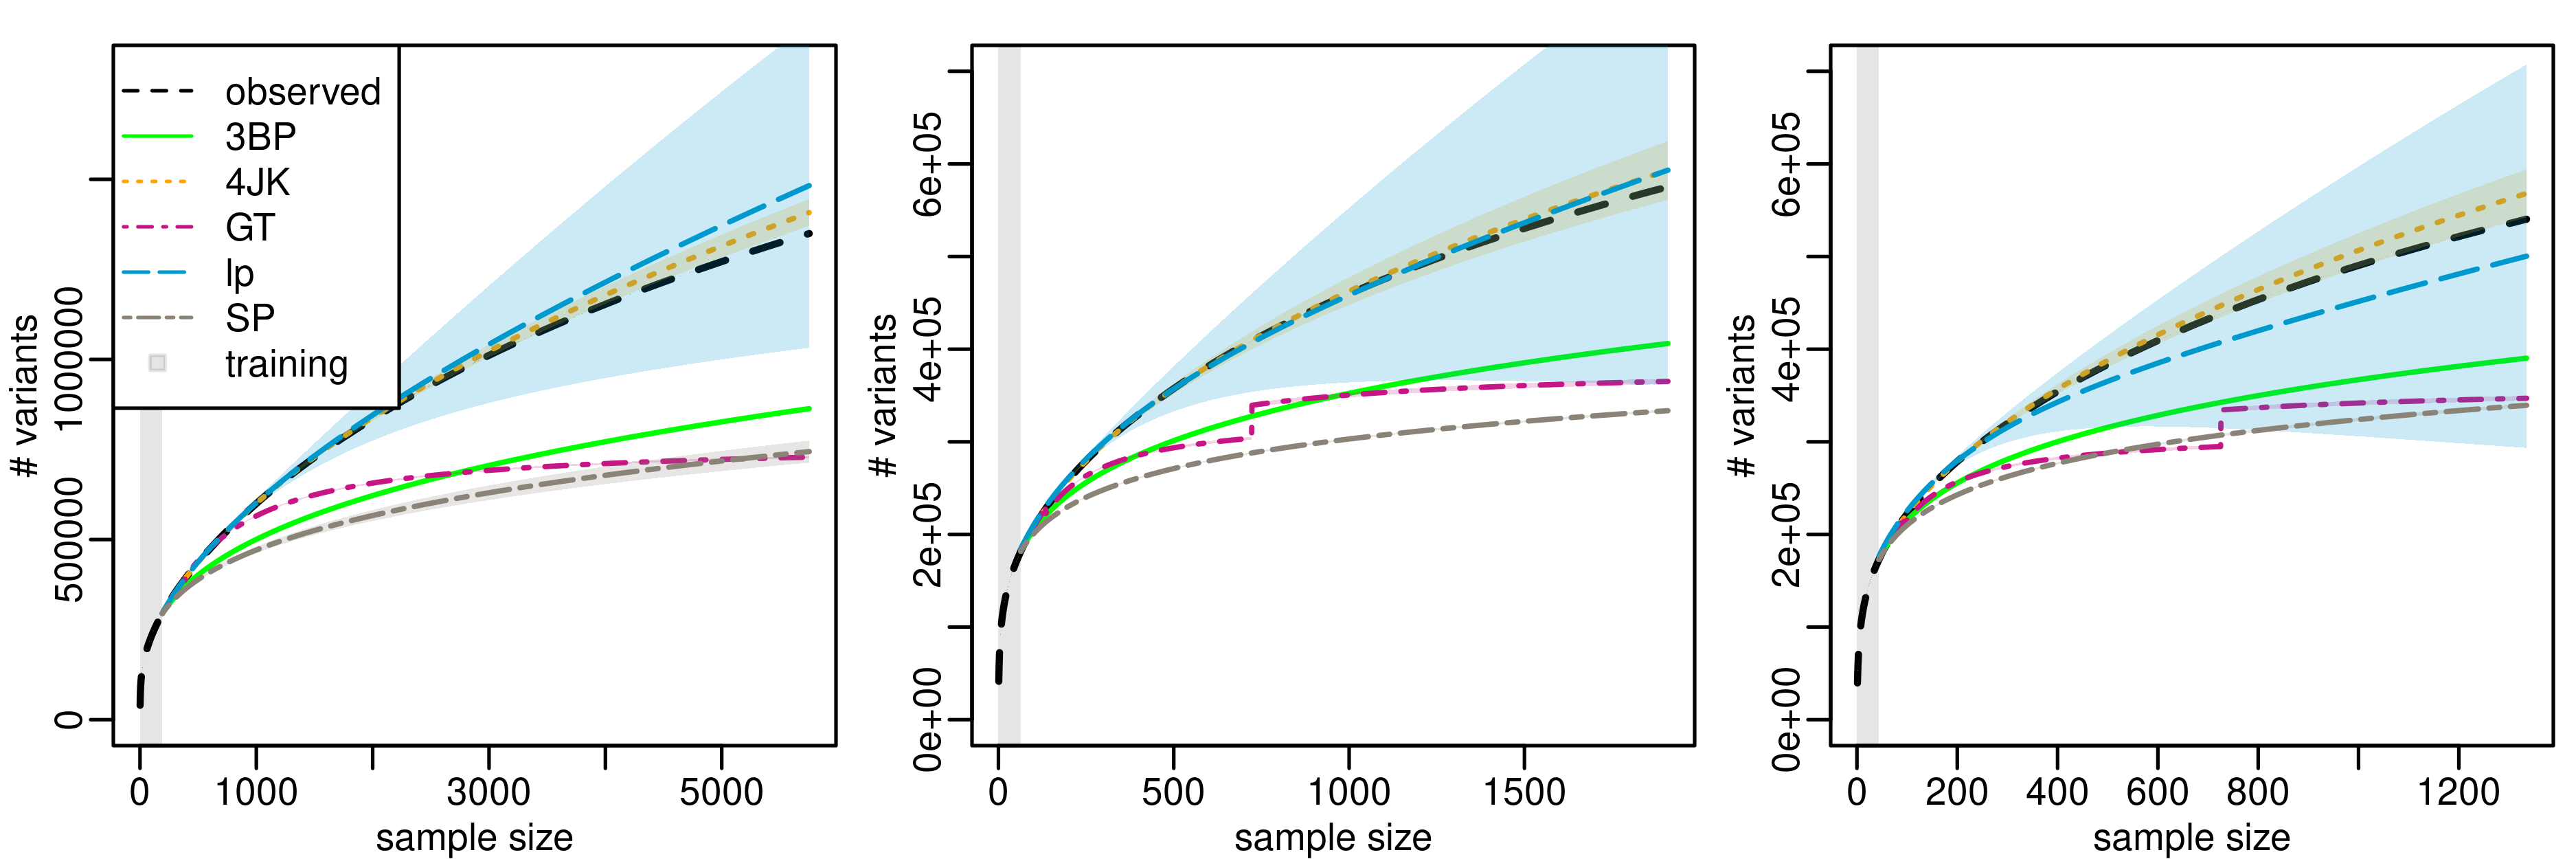
\includegraphics[width = 0.9\textwidth]{Ch2-double-trouble/Figs//Gnomad_one_pop_combined.png}
    \caption{Prediction for the GnomAD dataset, Left column: Southern European, Middle column: Korean,  Right column: Bulgarian. The dashed black line shows the observed number of variants as a function of the sample number. The samples appear in the following order: the pilot and then followup. The gray shading covers the
    pilot data. All curves agree exactly on the pilot data. In the follow-up region we plot mean (lines) and 1 standard deviation interval (shaded area) from five candidate single population models: 3BP (solid green), fourth order jackknife (dotted orange), GT (purple dot-line), linear programming (dashed cyan) and scaled process (dot dashed gray). The fourth order Jackknife outperforms competing alternatives in this dataset. 
    }
    \label{fig:seu_bgr_singlepop}
\end{figure}


\subsection{Raw number of shared variants and residuals in simulation and real data experiments}
\label{sec:raw_responses}

In this section, unlike in \cref{sec:single_pop_methods}, we report the raw number of shared variants and the raw magnitude of residuals (difference between predicted and true). Our findings when using this raw measure are similar to the ones obtained when using normalized residuals: our proposed methods performs well overall. 
We adopt the same ``cross-validation-like'' approach discussed in Section 8 (Experimental Setup).


\paragraph{Simulations}
%\label{sec:raw_responses_simulated}

In this section, we simulate data from our proposed model, following the approach discussed in \Cref{app:sample_from_pois}, the i3BP and the d3BP respectively. We test the predictive performance of our proposed model, as well as competing models on this data. 

For our proposed model, we simulate two datasets, using the following configuration of hyperparameters:
$(\mass,\rate{1}, \rate{2},\corr{1},\corr{2}, \conc{1}, \conc{2})=(100,0.4,0.6,0.5,0.5,1,1)$ and $(\mass,\rate{1}, \rate{2},\corr{1},\corr{2}, \conc{1}, \conc{2})=(1,0.8,0.7,0.5,0.5,1,1)$. We show the log raw number of ground truth and model predicted $\bm{k}$-tons in \cref{fig:proposed_kton}. 


\begin{figure}[H]
    \centering
    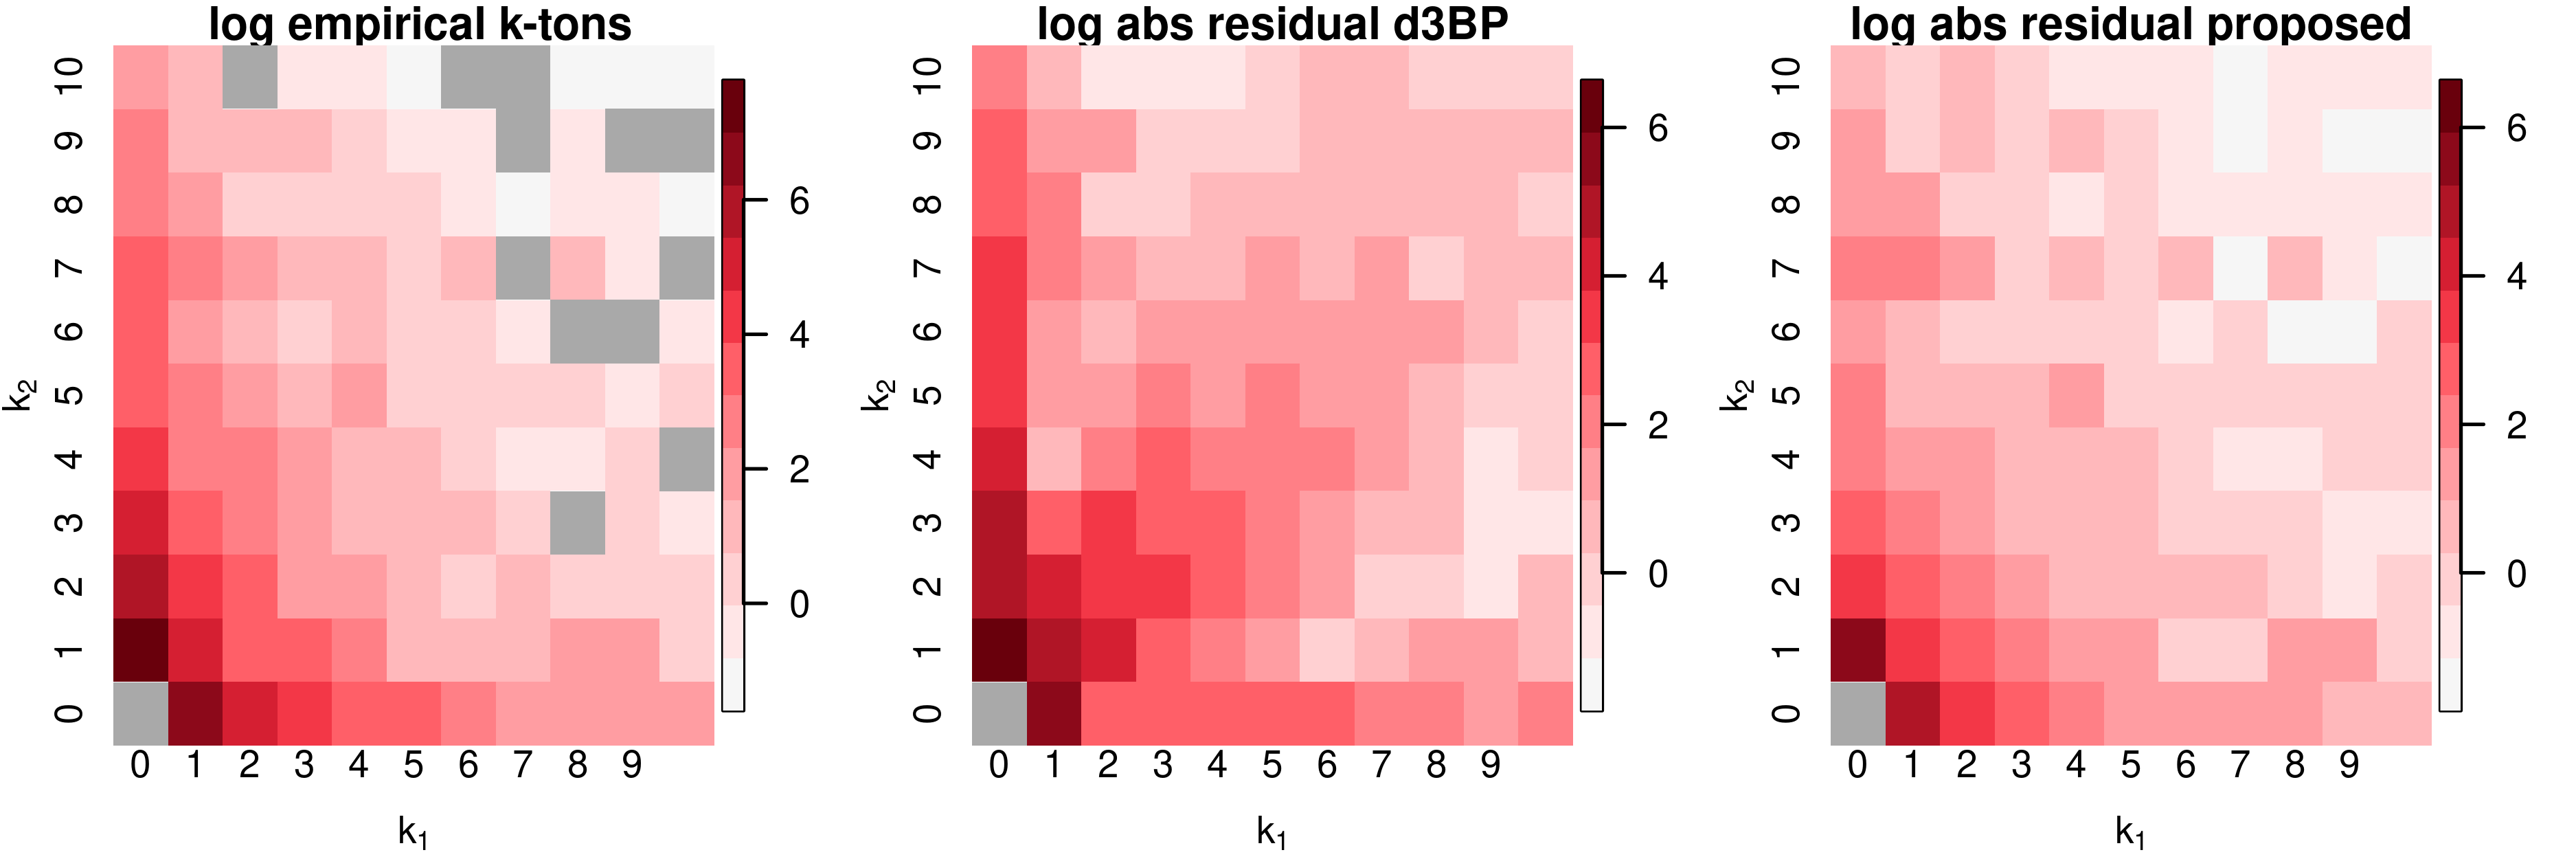
\includegraphics[width = 0.9\textwidth]{Ch2-double-trouble/Figs//n3bp_20fold_kton_res.png}
    \includegraphics[width = 0.9\textwidth]{Ch2-double-trouble/Figs//n3BP_fast_20fold_kton_res.png}
    \caption{Ground truth value of $\bm{k}$-tons and model prediction when the data is sampled from the proposed model. 
    Left most:log over average observed $\bm{k}$-tons. A square is gray when it the observed value is 0 in any fold or $\vecoccurrence=(0,0)$. Middle and right: Log average absolute residual in the d3BP and proposed model.  The first row refers to $(\mass,\rate{1}, \rate{2},\corr{1},\corr{2}, \conc{1}, \conc{2})=(100,0.4,0.6,0.5,0.5,1,1)$. The second row refers to $(\mass,\rate{1}, \rate{2},\corr{1},\corr{2}, \conc{1}, \conc{2})=(1,0.8,0.7,0.5,0.5,1,1)$.
    }
    \label{fig:proposed_kton}
\end{figure}



For the i3BP, we simulate two datasets using parameters $(\alpha_1,c_1,\sigma_1,\alpha_2,c_2,\sigma_2) = (20,1,.6,20,1,.3)$, and $(\alpha_1,c_1,\sigma_1,\alpha_2,c_2,\sigma_2)=(40,1,.1,40,1,.3)$. We show the log raw number of ground truth and model predicted $\bm{k}$-tons in \cref{fig:i3BP_kton}. 

\begin{figure}[H]
    \centering
    \includegraphics[width = 0.9\textwidth]{Ch2-double-trouble/Figs//i3BP_20fold_kton_res.png}
    \includegraphics[width = 0.9\textwidth]{Ch2-double-trouble/Figs//i3BP_slow_20fold_kton_res.png}
    \caption{Ground truth of $\bm{k}$-tons and model prediction when the data sampled from the i3BP. Left most:log over average observed $\bm{k}$-tons. A darker color corresponds to higher values. A square is gray when it the observed value is 0 in any fold or $\vecoccurrence=(0,0)$. Middle and right: Log average absolute residual in the d3BP and the proposed model.  The first row refers to $(\alpha_1,c_1,\sigma_1,\alpha_2,c_2,\sigma_2) = (20,1,.6,20,1,.3)$. The second row refers to $(\alpha_1,c_1,\sigma_1,\alpha_2,c_2,\sigma_2)=(40,1,.1,40,1,.3)$.
    }
    \label{fig:i3BP_kton}
\end{figure}


For the d3BP, we simulated two datasets using parameters $(\alpha,c,\sigma)=(20,1,.5)$, and $(\alpha,c,\sigma)=(40,1,.1)$. We showed the log raw number of ground truth and model predicted $\bm{k}$-tons in \cref{fig:d3BP_kton}. 


\begin{figure}[H]
    \centering
    \includegraphics[width = 0.9\textwidth]{Ch2-double-trouble/Figs//d3BP_20fold_kton_res.png}
    \includegraphics[width = 0.9\textwidth]{Ch2-double-trouble/Figs//d3BP.1_20fold_kton_res.png}
    \caption{Ground truth of $\bm{k}$-tons and model prediction when the data sampled from the d3BP. Left most:log over average observed $\bm{k}$-tons. A darker color corresponds to higher values. A square is gray when it the observed value is 0 in any fold or $\vecoccurrence=(0,0)$. Middle and right: Log average absolute residual in the d3BP and the proposed model. The first row refers to $(\alpha,c,\sigma)=(20,1,.5)$. The second row refers to $(\alpha,c,\sigma)=(40,1,.1)$.}
    \label{fig:d3BP_kton}
\end{figure}

\subsection{Real data experiment}

\Cref{fig:brca_luad_kton} and~\cref{fig:seu_bgr_kton} show the raw number of $\bm{k}$-tons that exist more than twice in all folds of cross-validations and the magnitude of raw residuals with real data. Again, we observe that predictions stemming from the d3BP tend to incur in larger residuals around the ``diagonal'' (same occurrences in both populations). This is consistent with the assumption made by the d3BP that variants share the same frequencies across populations. 

\begin{figure}[H]
    \centering
    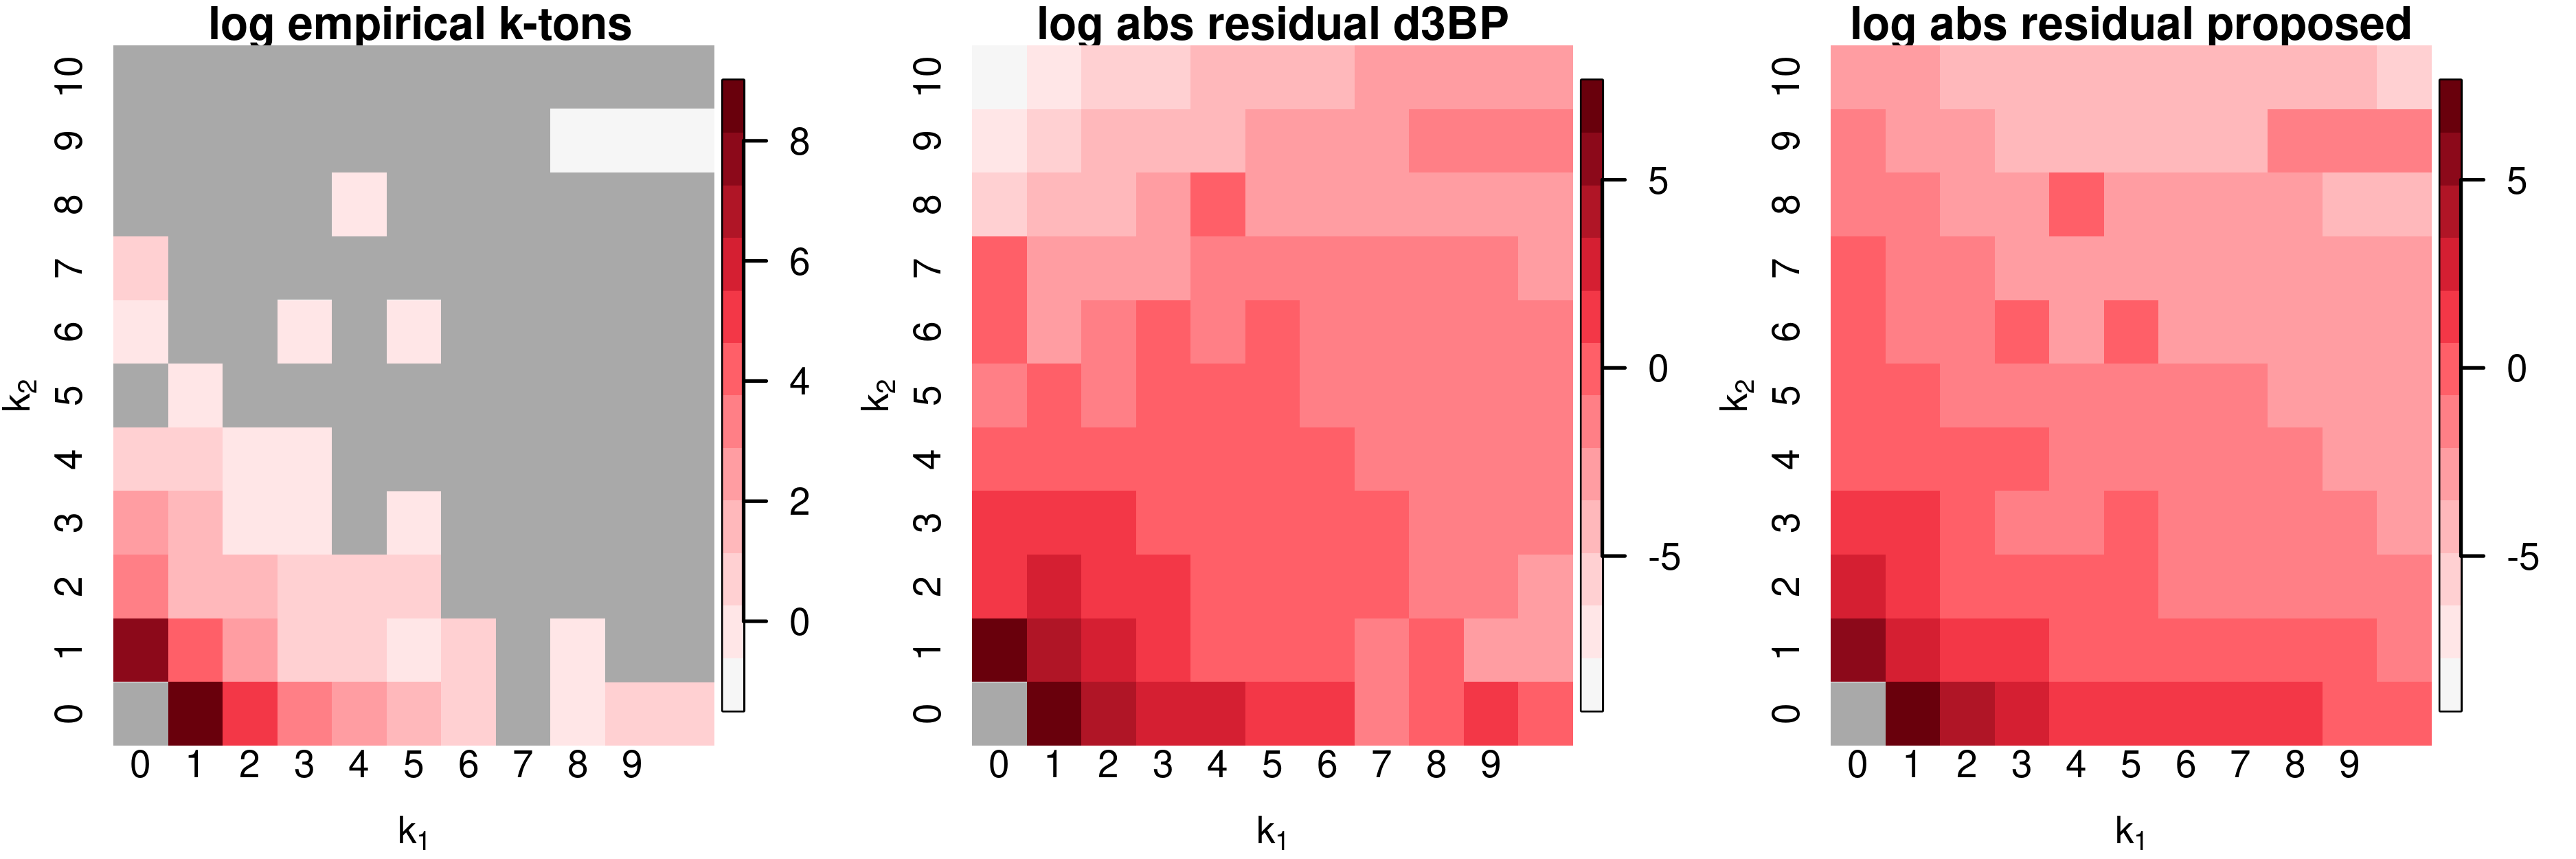
\includegraphics[width = 0.9\textwidth]{Ch2-double-trouble/Figs//BIDC_LA2_20fold_kton_res.png}
    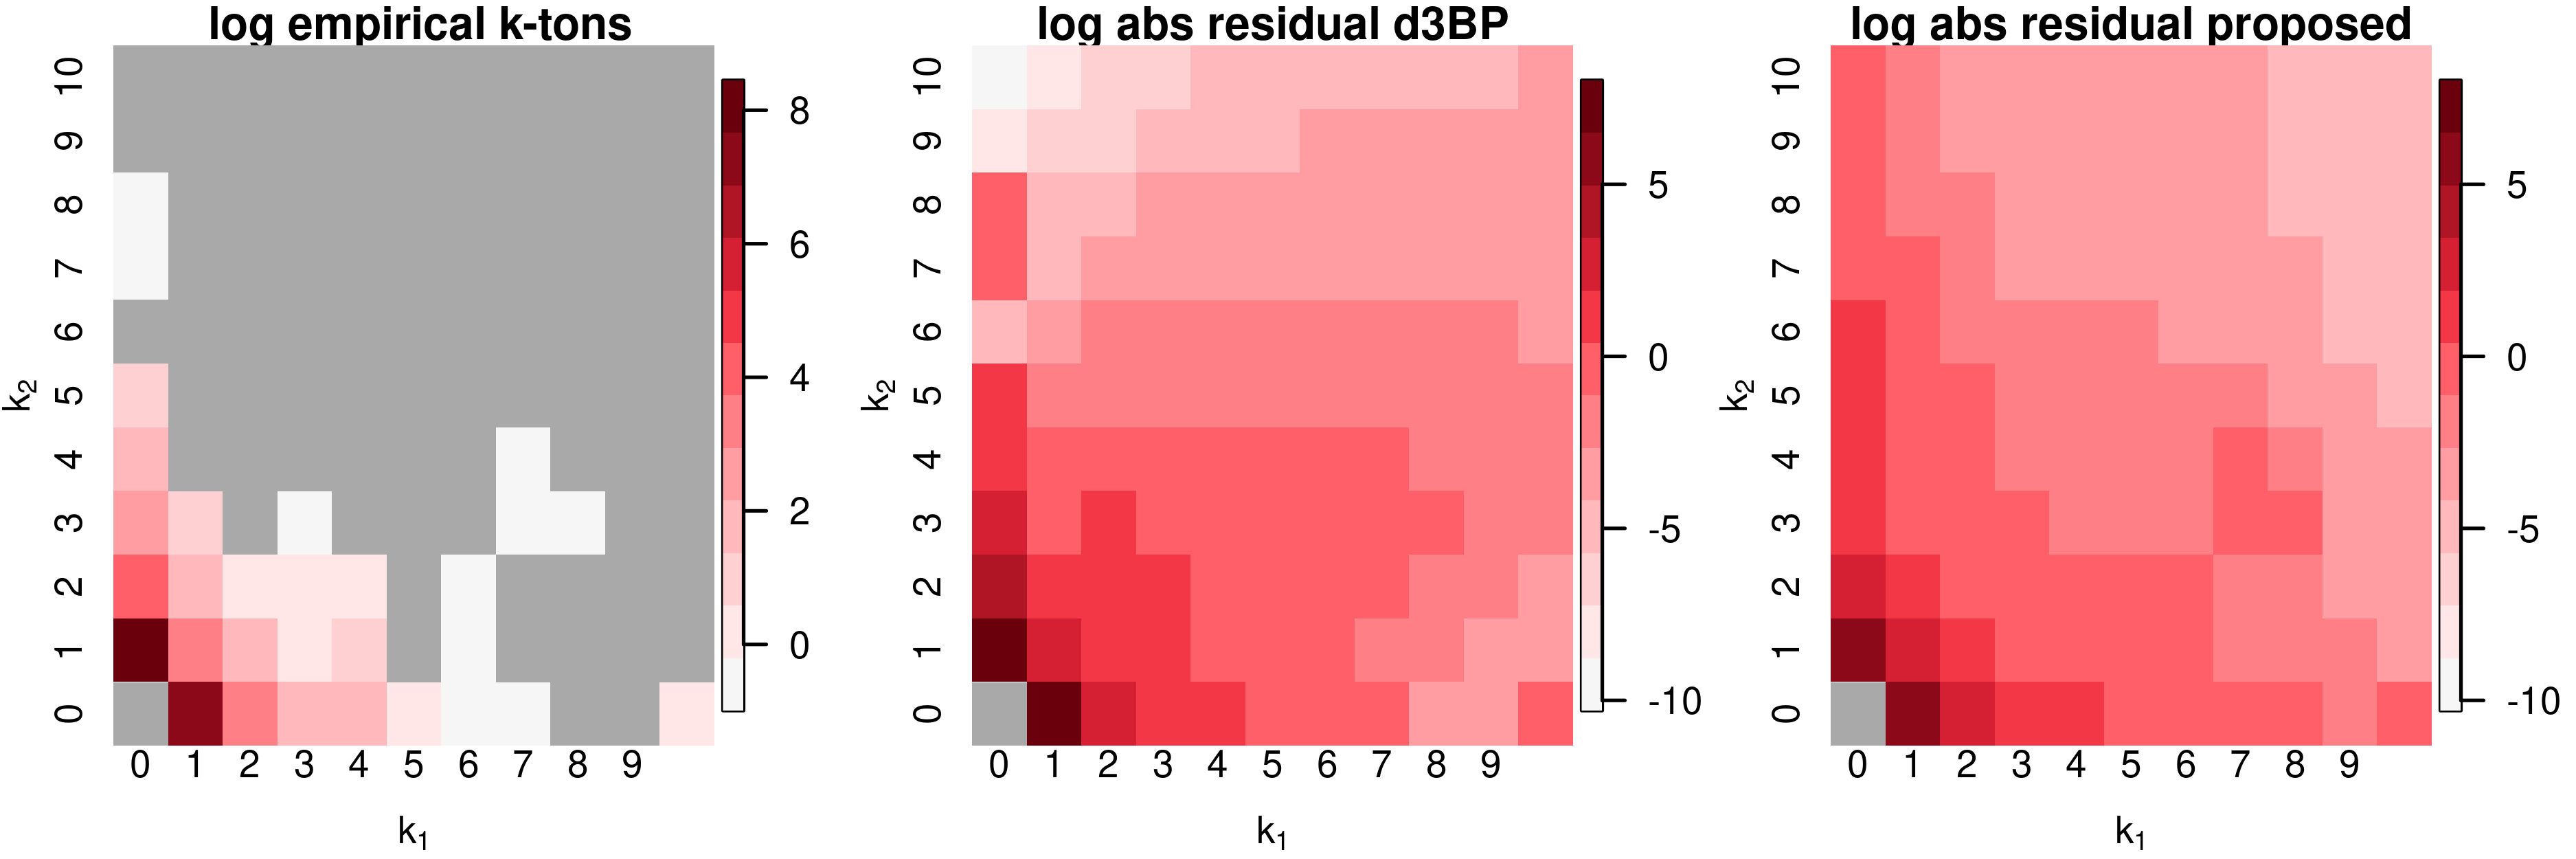
\includegraphics[width = 0.9\textwidth]{Ch2-double-trouble/Figs//BRCA_LUAD_20fold_kton_res.png}
    \caption{Ground truth of $\bm{k}$-tons and model prediction using cancer genome dataset. Left most:log over average observed $\bm{k}$-tons. A darker color corresponds to higher values. A square is gray when it the observed value is 0 in any fold or $\vecoccurrence=(0,0)$. Middle and right: Log average absolute residual in d3BP and proposed model. }
    %\label{fig:brca_luad_kton}
    \label{fig:brca_luad_kton}
\end{figure}


\begin{figure}[H]
    \centering
    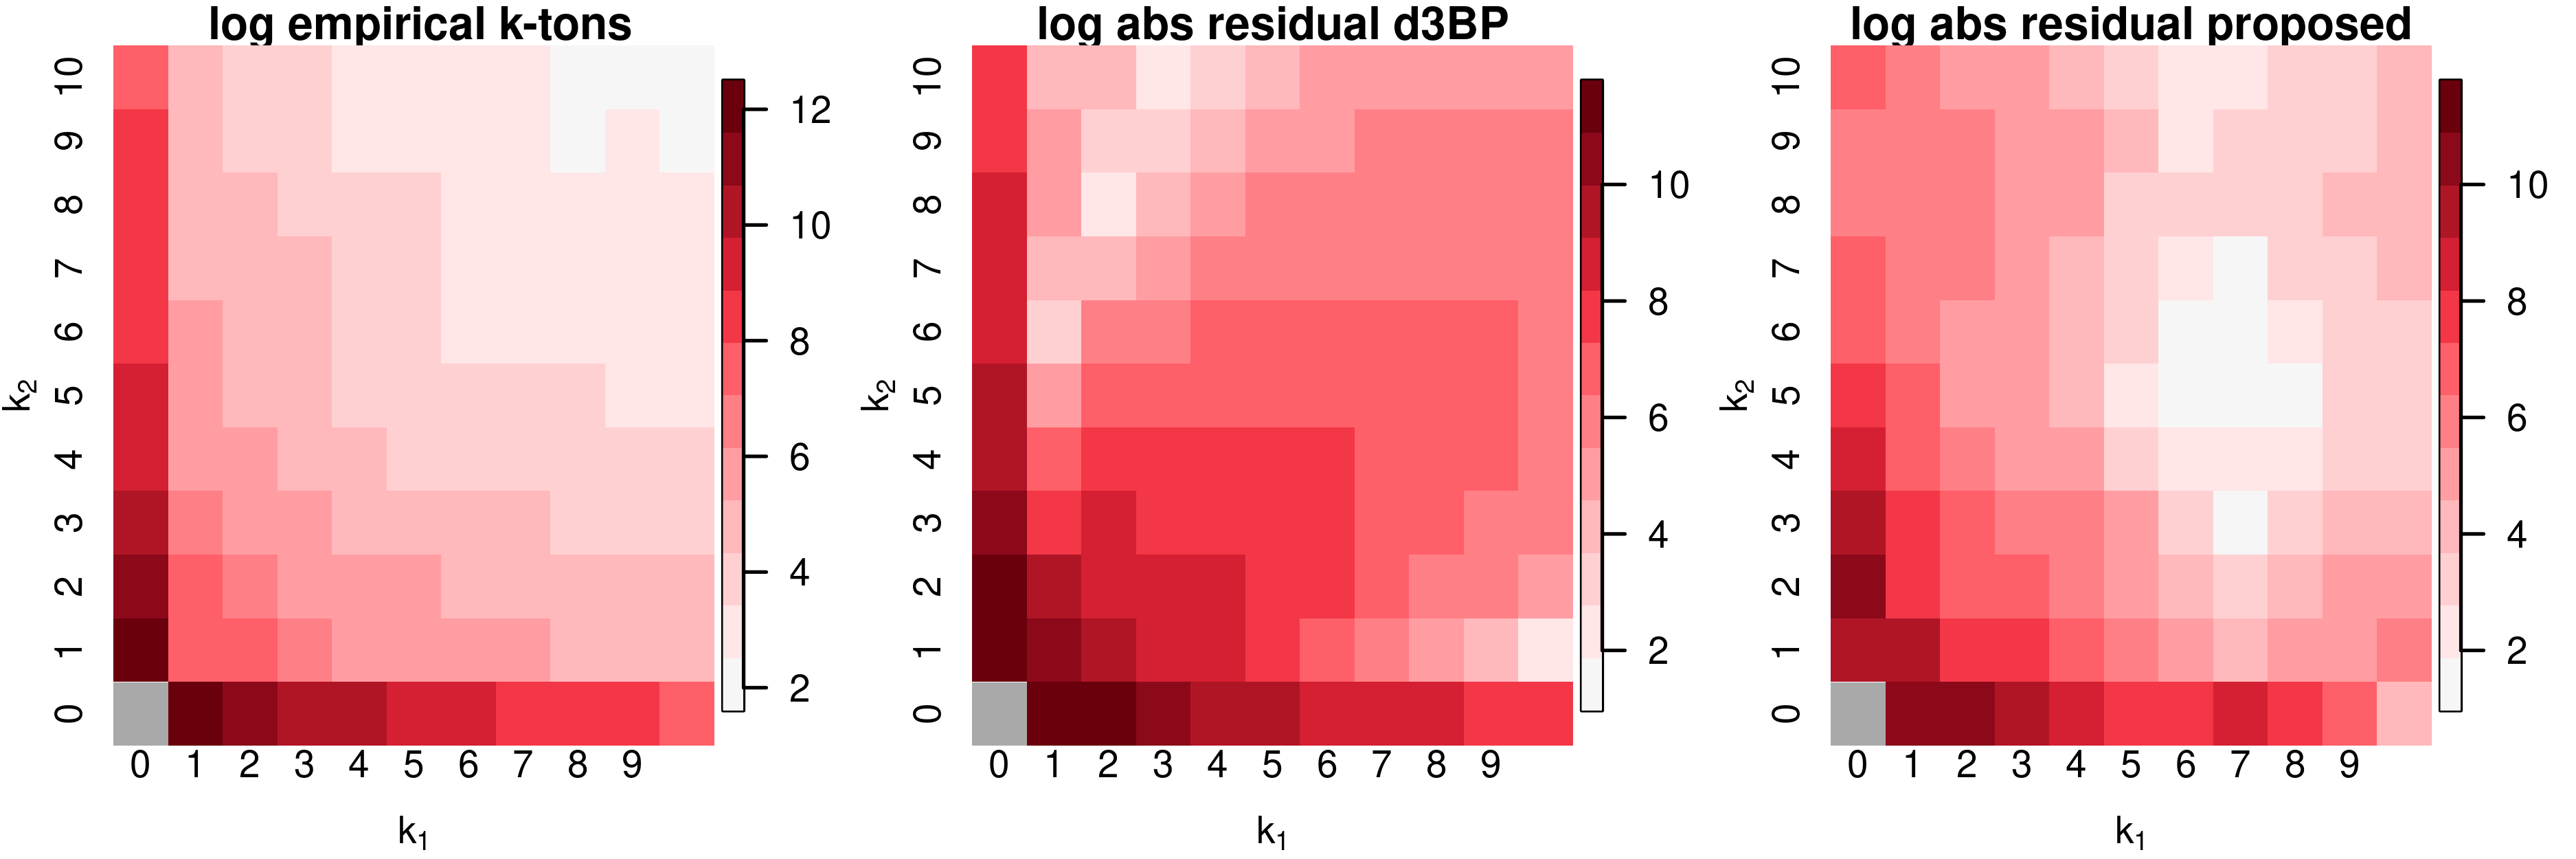
\includegraphics[width = 0.9\textwidth]{Ch2-double-trouble/Figs//kor_bgr_30fold_kton_res.png}
    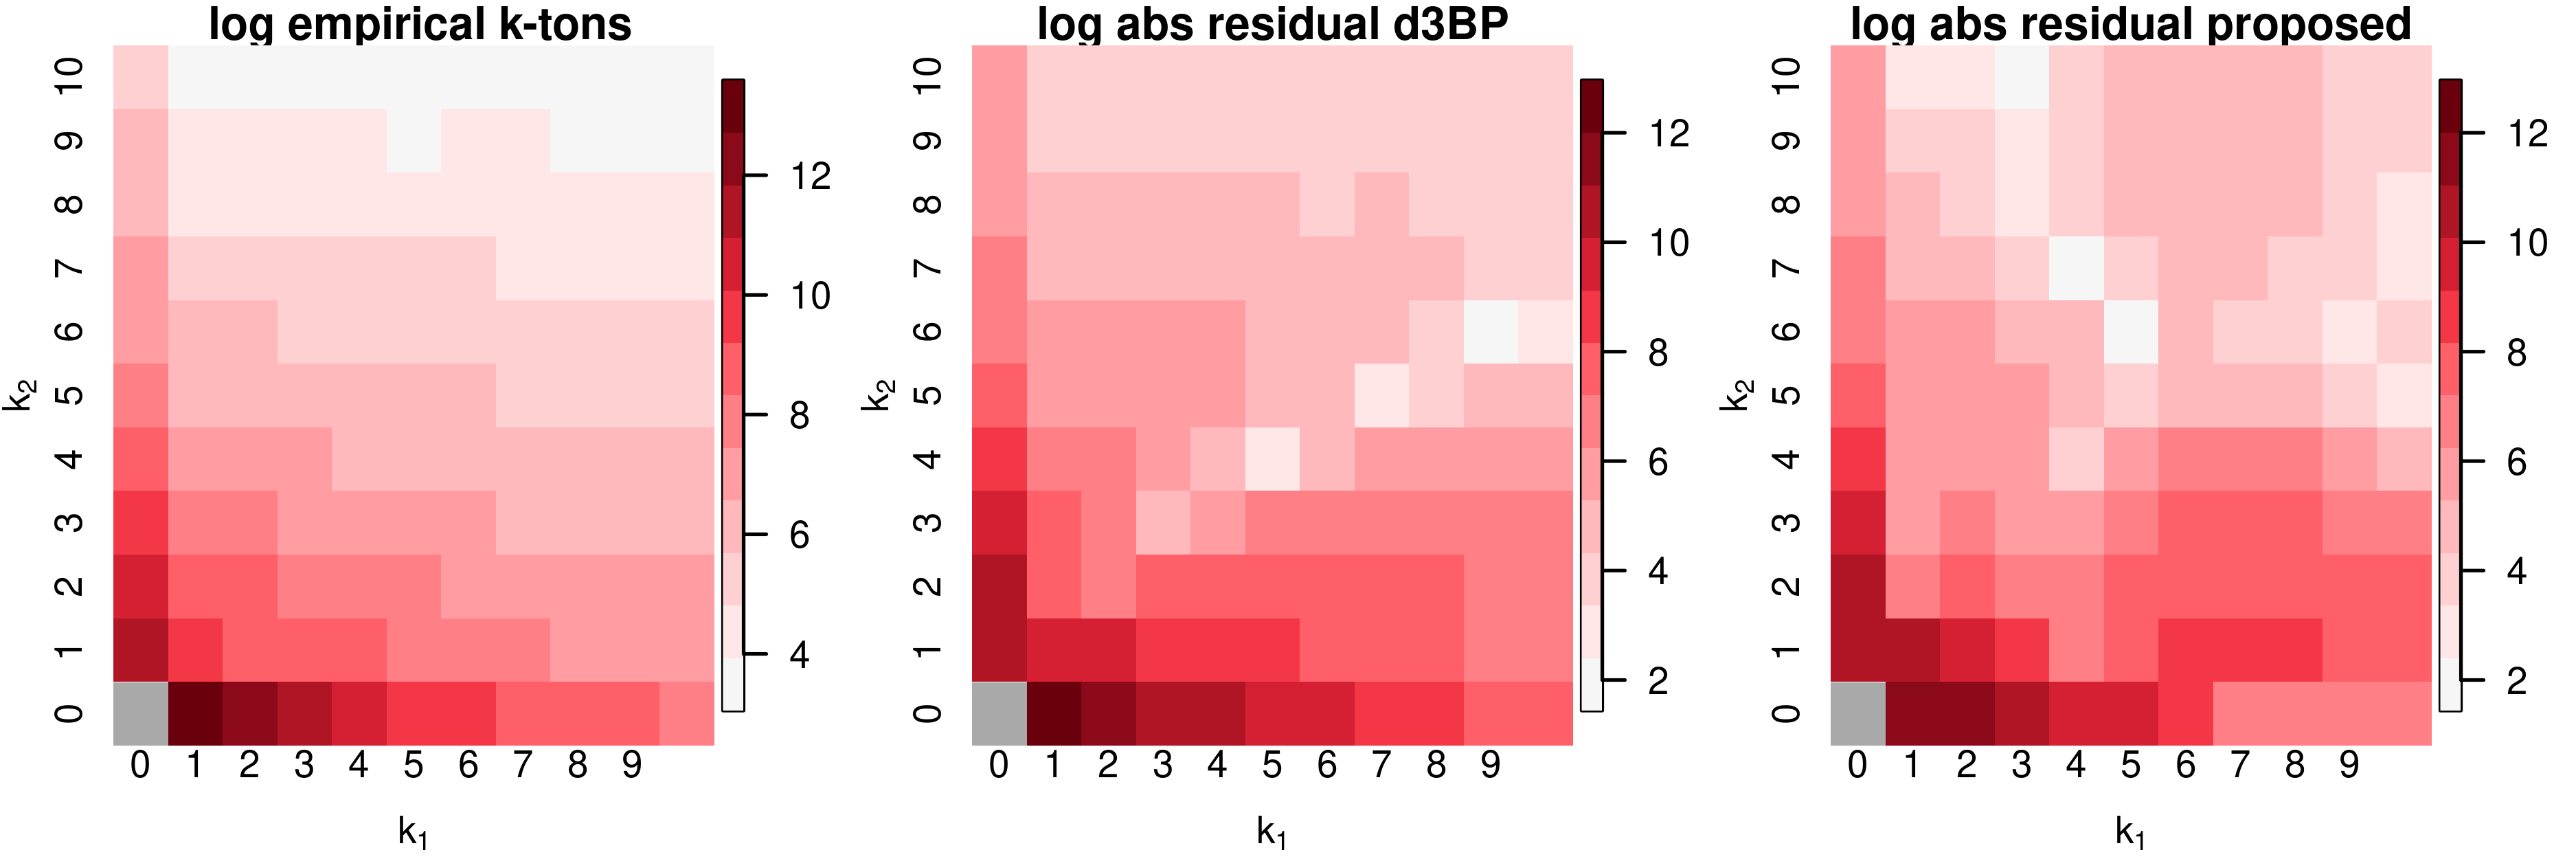
\includegraphics[width = 0.9\textwidth]{Ch2-double-trouble/Figs//seu_bgr_30fold_kton_res.png}
    \caption{Ground truth of $\bm{k}$-tons and model prediction using GnomAD dataset. Left most:log over average observed $\bm{k}$-tons. A darker color corresponds to higher values. A square is gray when it the observed value is 0 in all fold or $\vecoccurrence=(0,0)$. Middle and right: Log average absolute residual in d3BP and proposed model. }
    %\label{fig:seu_bgr_kton}
    \label{fig:seu_bgr_kton}
\end{figure}

\subsection{Our method avoids double counting when the number of variants grows slowly}
\label{sec:slow_growth}

In this section, we show our model's behavior when fitted to data generated by a d3BP with low power law rate, or generated by the proposed model again with low power law rates. 
Our proposed method handles well both cases. Conversely, the i3BP can induce severe double counting of predicted variants.

\begin{figure}[H]
    \centering
    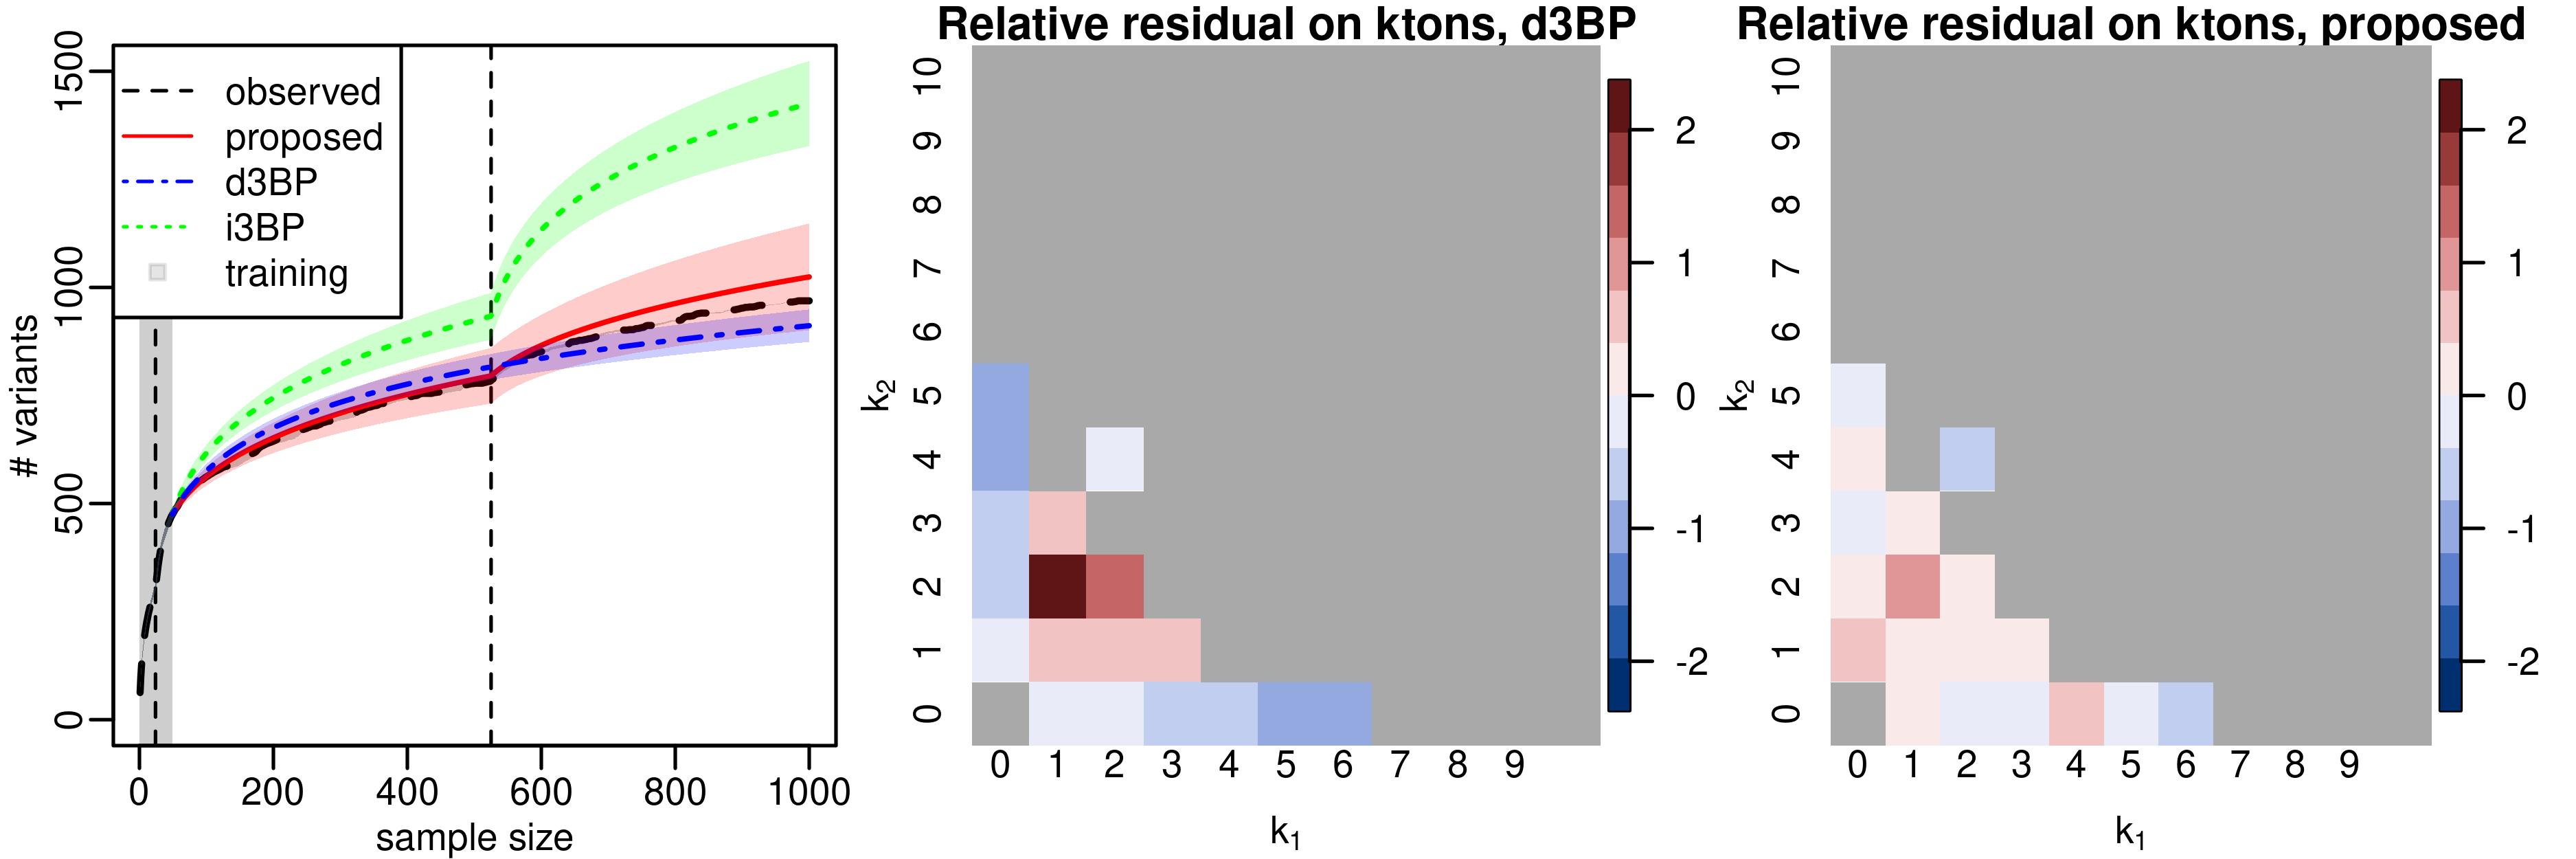
\includegraphics[width = 0.9\textwidth]{Ch2-double-trouble/Figs//n3bp_slow_20fold.png}
    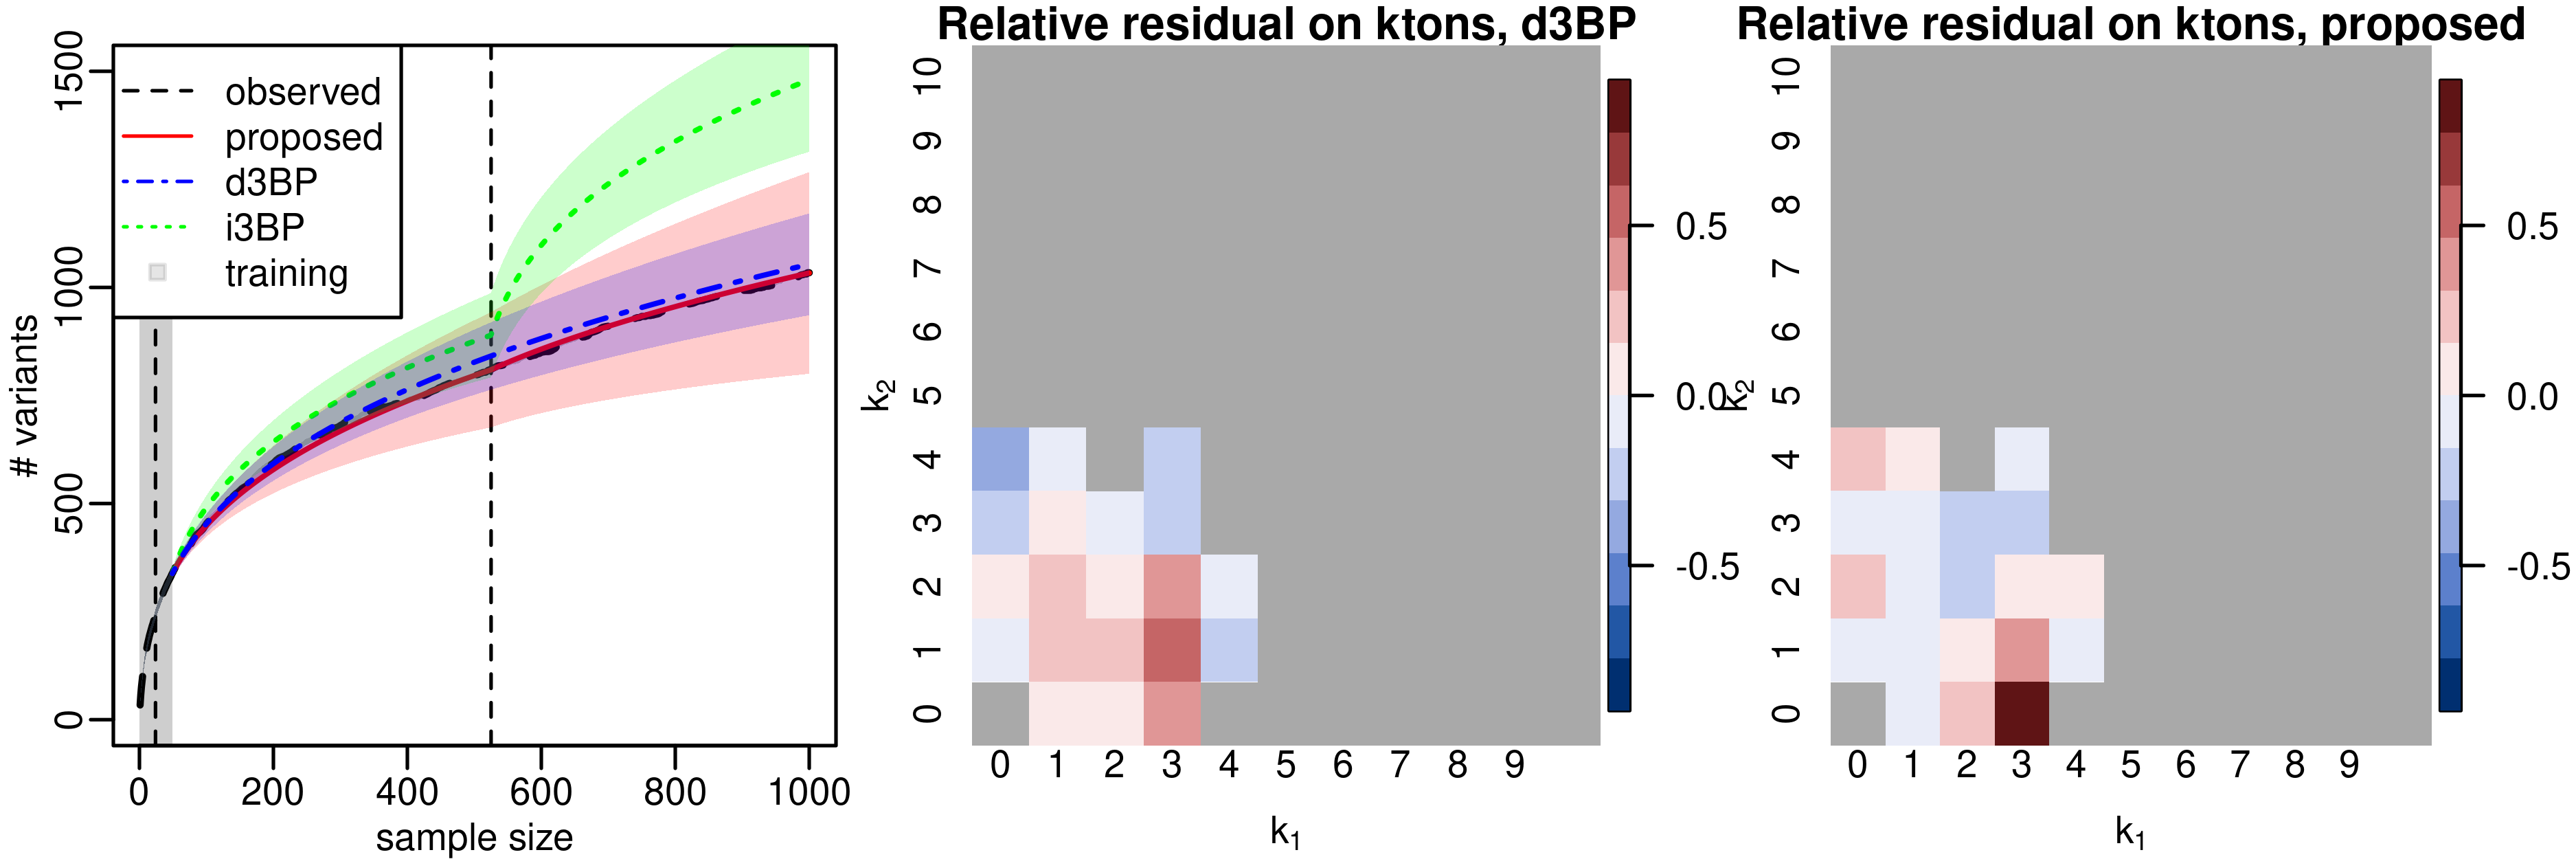
\includegraphics[width = 0.9\textwidth]{Ch2-double-trouble/Figs//d3bp.3_20fold.png}
    \caption{Prediction for slow growth correlated models. Top: proposed model $(\mass,\rate{1}, \rate{2}, \corr{1}, \corr{2}, \discount{1}, \discount{2})=(100,0.4,0.6,0.5,0.5,1,1)$. Bottom: d3BP $(\alpha,c,\sigma)=(40,1,.3)$. The dashed black line shows the observed number of variants as a function of the sample number. The samples appear in the following order: the pilot and then followup. The gray shading covers the
    pilot data. All curves agree exactly on the pilot data. In the follow-up region we plot mean (lines) and 1 standard deviation interval (shaded area) from five candidate single population models: 3BP (solid green), fourth order jackknife (dotted orange), GT (purple dot-line), linear programming (dashed cyan) and scaled process (dot dashed gray). }
    \label{fig:slow_growth}
\end{figure}


\subsection{Larger trimming during training}
\label{sec:large_triming}
In Section 6.2 we discussed how the estimation of our model's hyperparameters involves maximizing the model's likelihood over a trimmed selection of $\bm{k}$-tons. 
In principle, one could be worried that our estimates are sensitive to our choice of the trimming threshold $\bm{k}$. We here present additional results, where we allow for larger trimming thresholds ($\bm{k}=(15,15)$ and $\bm{k} = (20,20)$) in the GnomAD and MSK-IMPACT dataset. 
Our results show that the optimization is relatively insensitive to the trimming threshold (Fig.~\ref{fig:seu_bgr_15}~\ref{fig:seu_bgr_20}~\ref{fig:bidc_la2_15}). 

\begin{figure}[H]
    \centering
    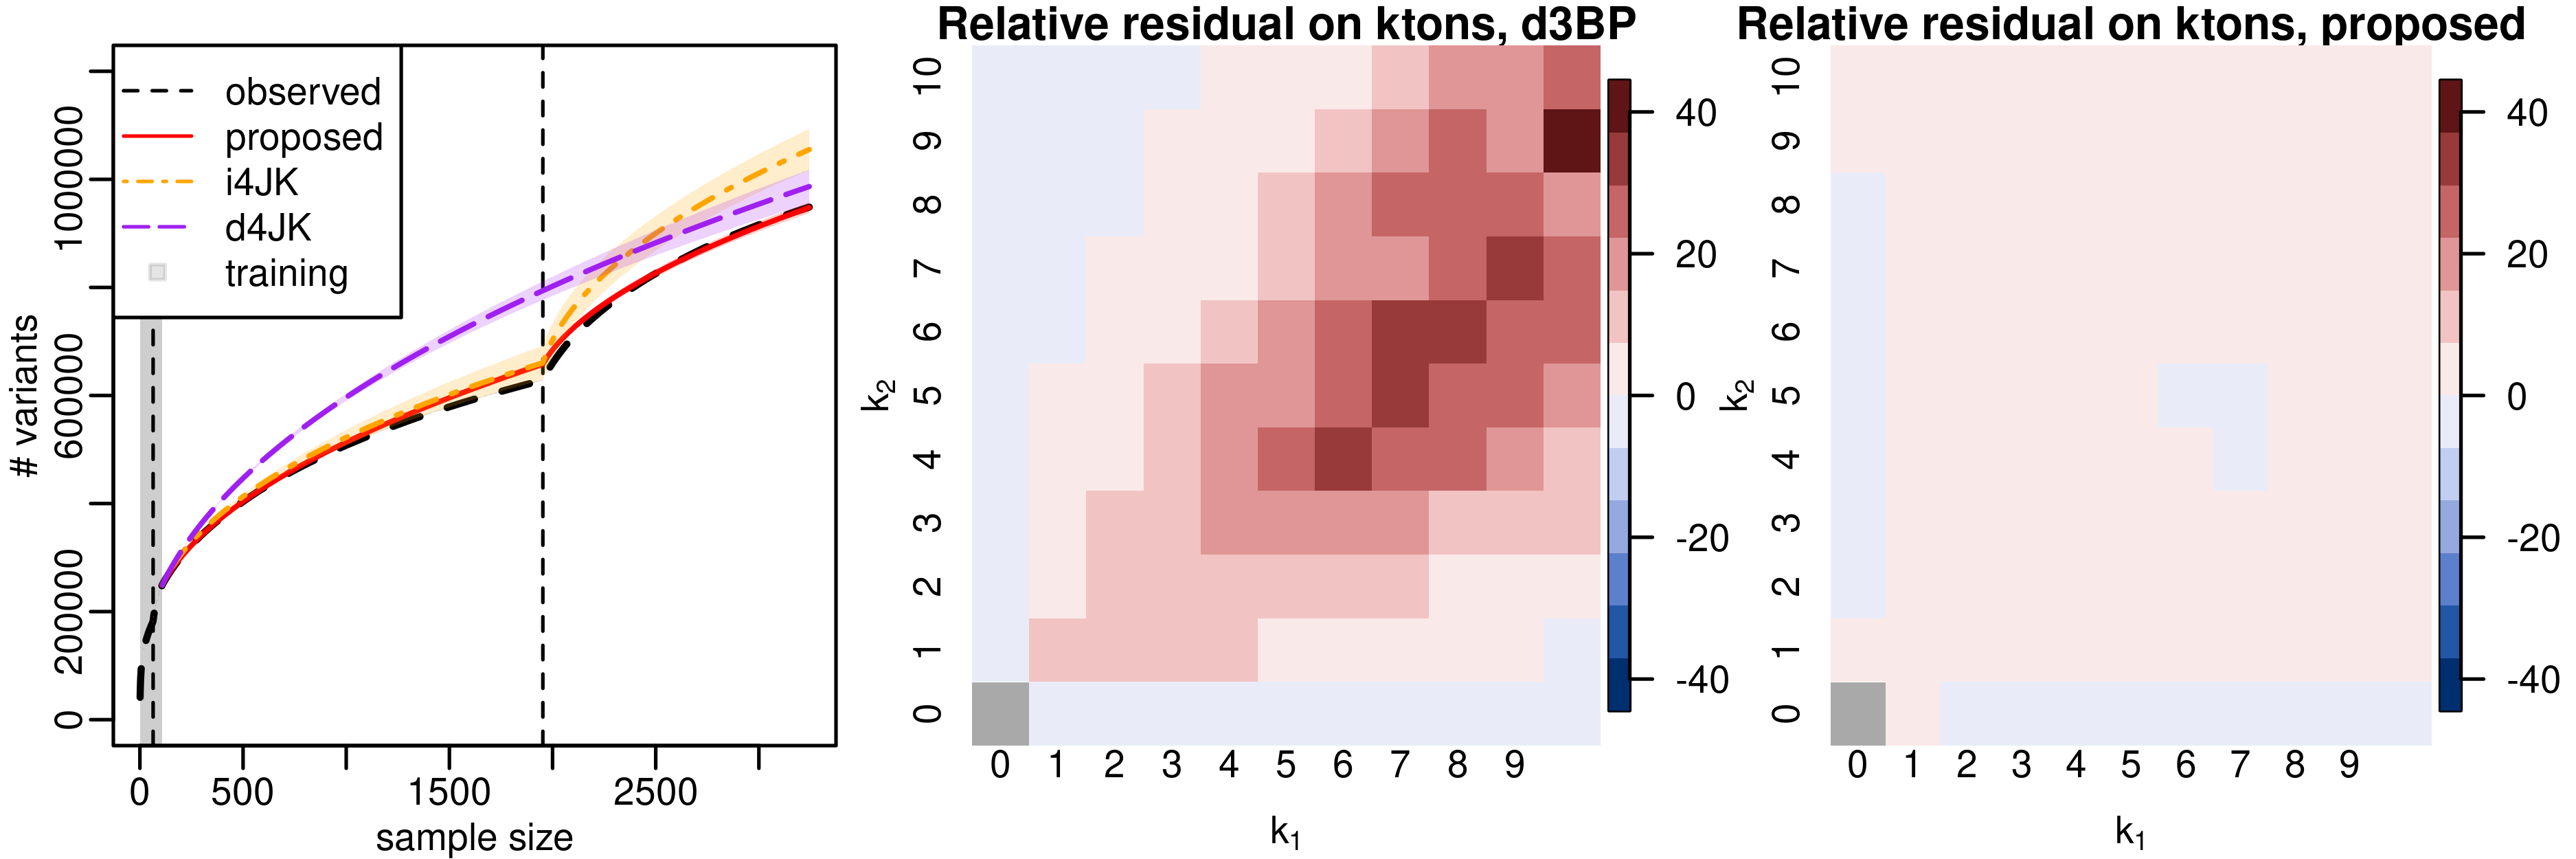
\includegraphics[width = 0.9\textwidth]{Ch2-double-trouble/Figs//kor_bgr_30fold_trim15.png}
    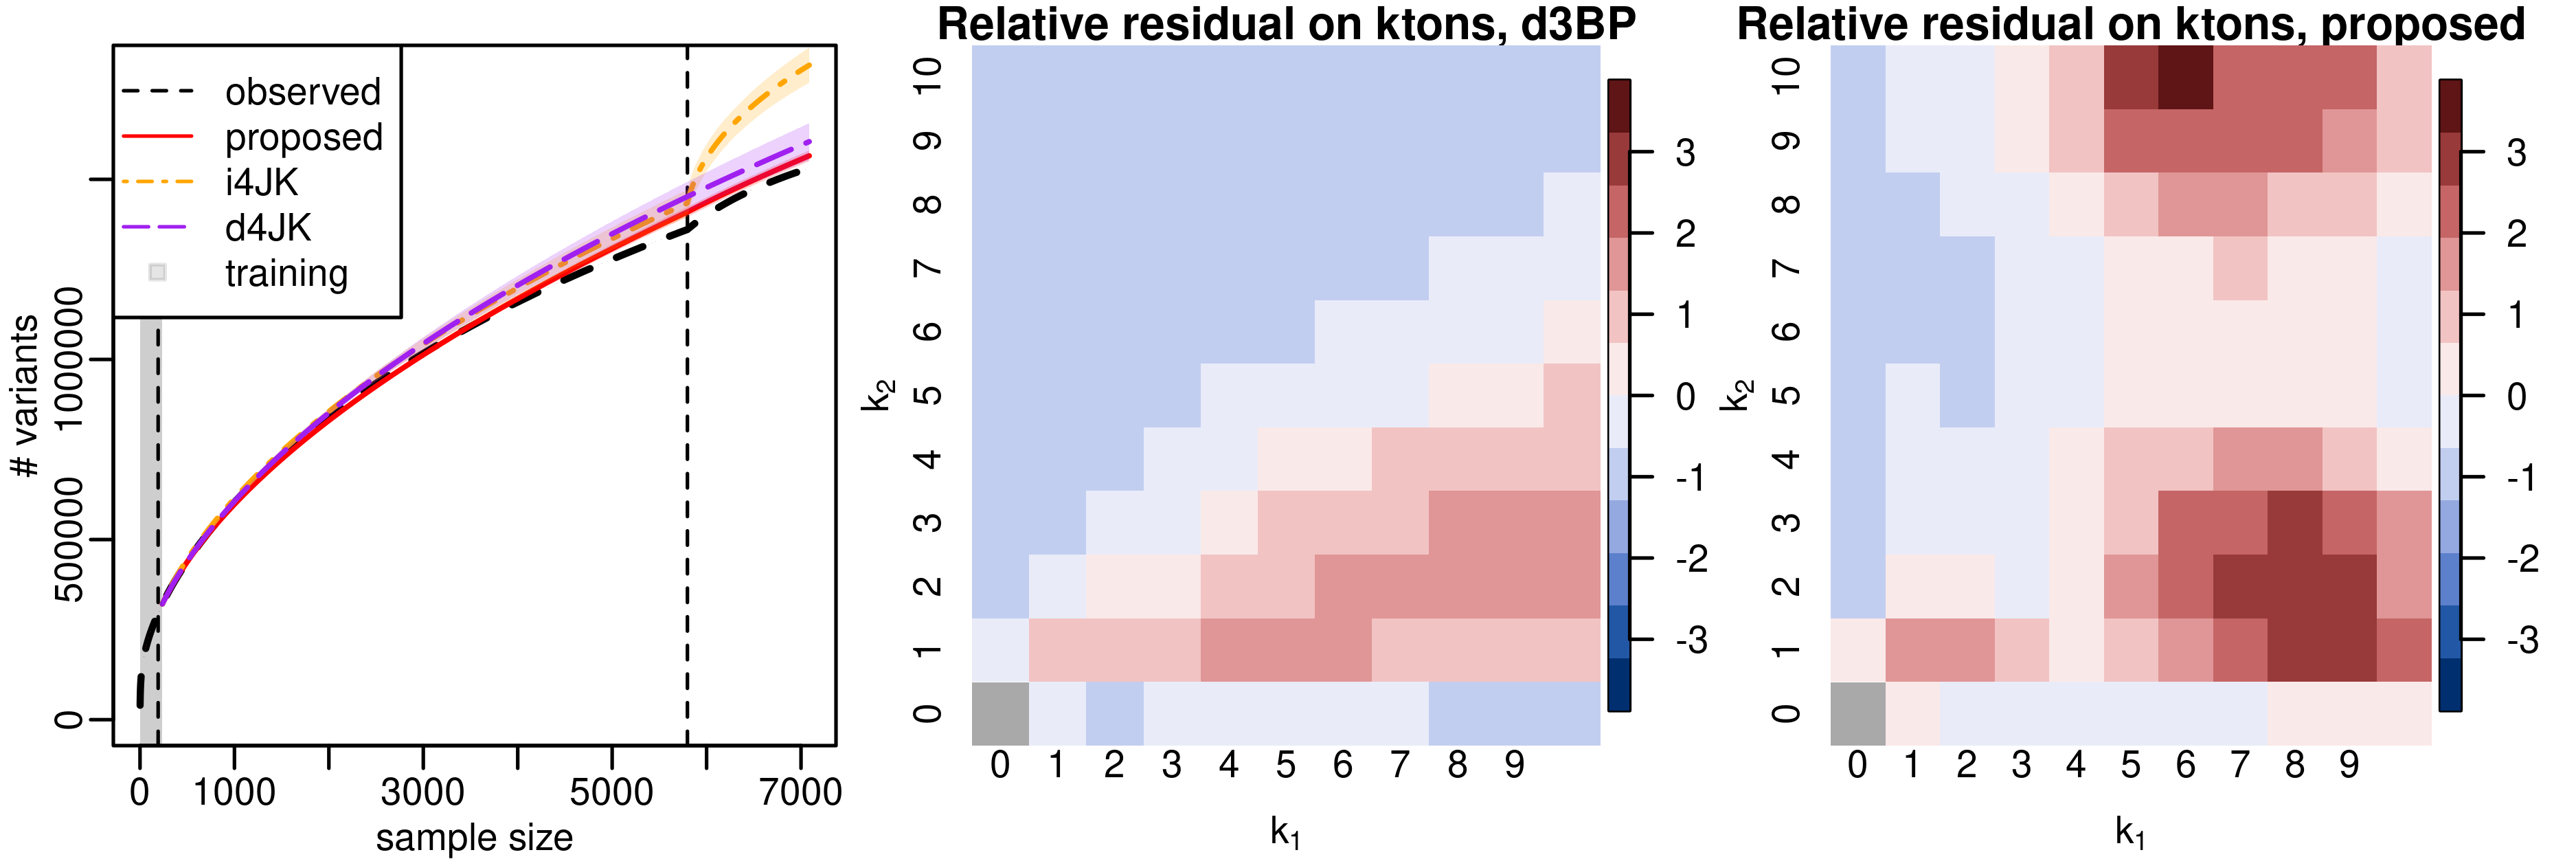
\includegraphics[width = 0.9\textwidth]{Ch2-double-trouble/Figs//seu_bgr_30fold_trim15.png}
    \caption{Prediction for the GnomAD dataset, Korean--Bulgarian and Southern European--Bulgarian respectively. The trimming here is set to 15. The results are the same as trimming at 10 in \cref{fig:pop_gen}.}
    %\label{fig:seu_bgr_15}
    \label{fig:seu_bgr_15}
\end{figure}

\begin{figure}[H]
    \centering
    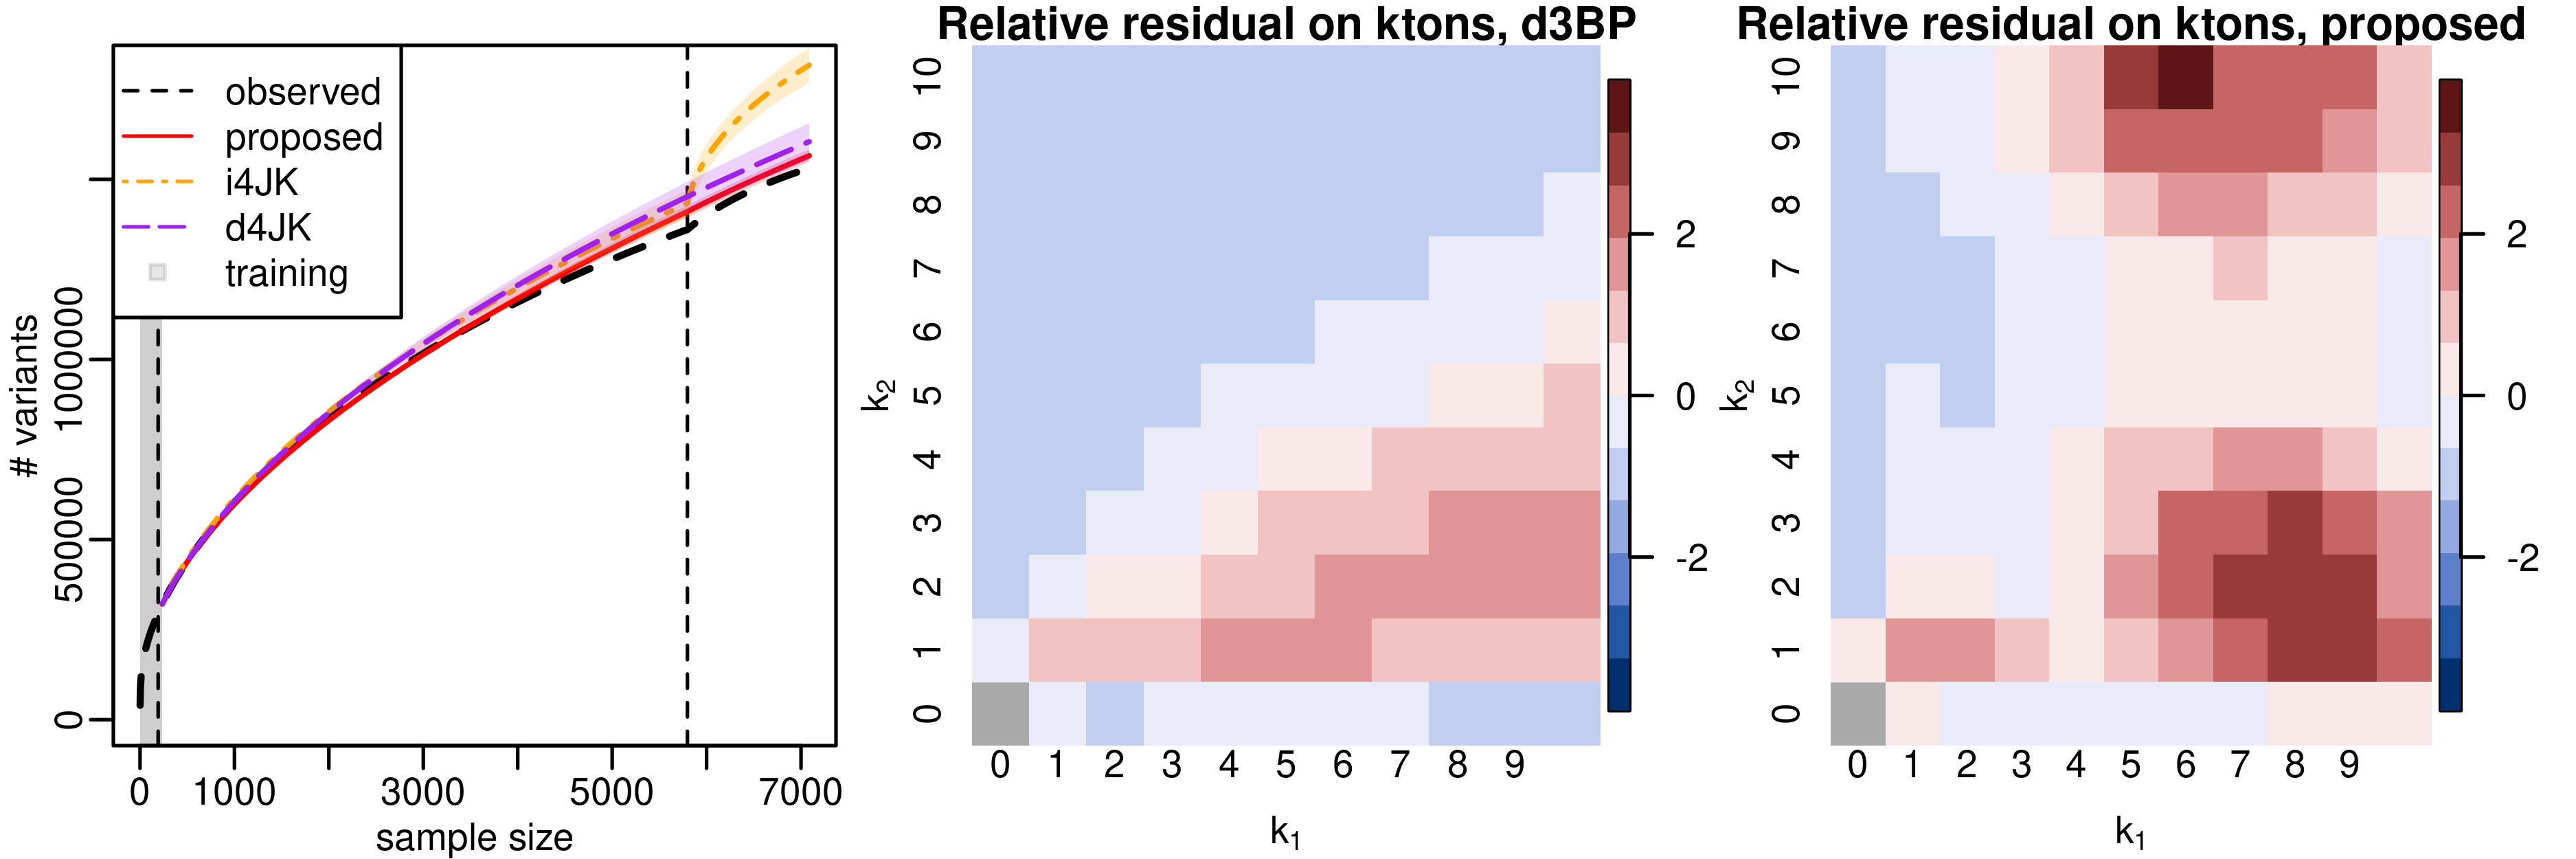
\includegraphics[width = 0.9\textwidth]{Ch2-double-trouble/Figs//seu_bgr_30fold_trim20.png}
    \caption{Prediction for the GnomAD dataset Southern European--Bulgarian respectively. The trimming here is set to 20. The results are the same as trimming at 10 in the \cref{fig:pop_gen}. The Korean population does not have enough training samples to allow a trimming of 20.}
    \label{fig:seu_bgr_20}
\end{figure}

\begin{figure}[H]
    \centering
    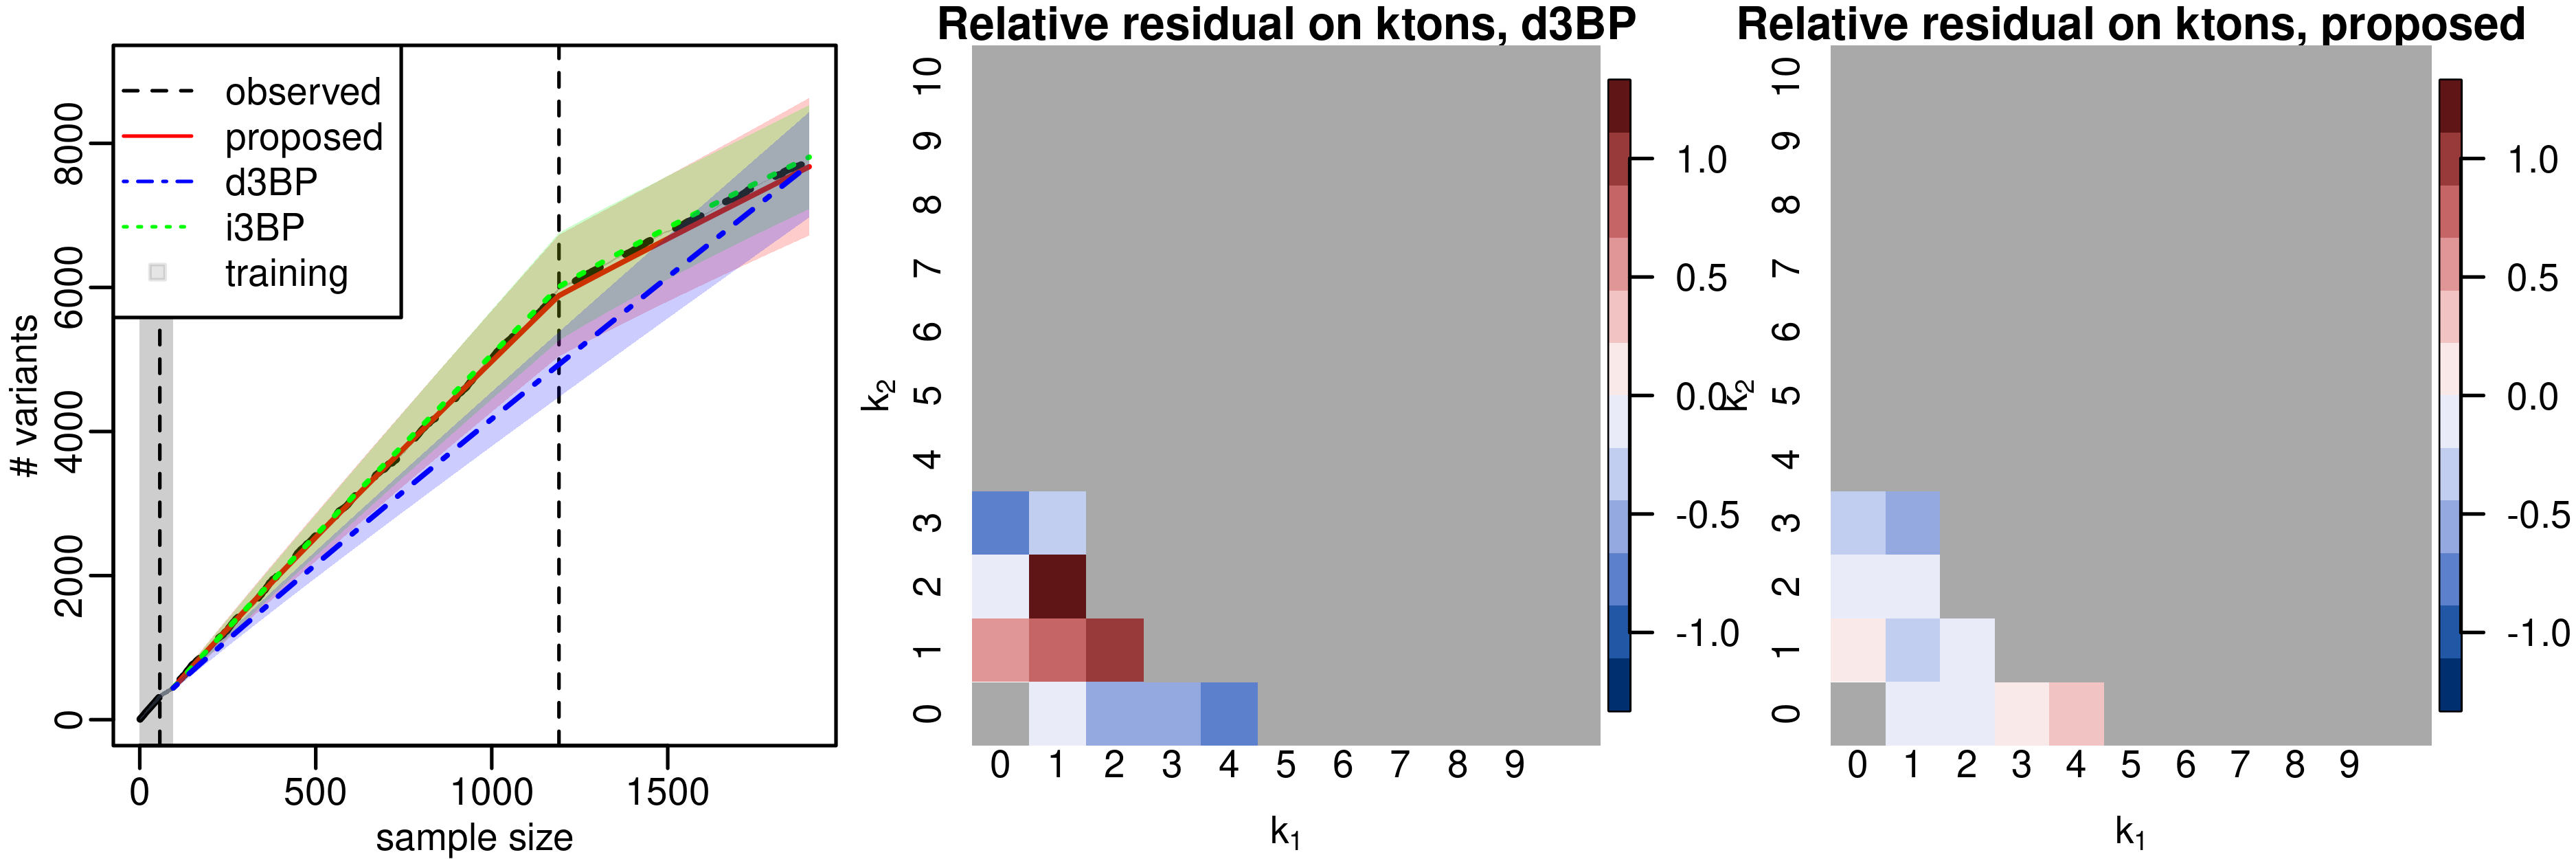
\includegraphics[width = 0.9\textwidth]{Ch2-double-trouble/Figs//BIDC_LA2_20fold_trim15.png}
    \caption{Prediction for the variant counts in, breast and lung cancer. For  MSK-IMPACT dataset. This experiment used trimming of 15 during training. The results are the same as trimming at 10 in the \cref{fig:cancer}.}
    \label{fig:bidc_la2_15}
\end{figure}


\paragraph{\revision{Why trimming with fixed size.}}
\revision{The key observation that underlies our truncation is the following: biologists are interested in predicting the number of new variants in the follow-up study. By construction, variants that are new in the follow-up did not appear in the pilot and therefore can be expected to have a low frequency (i.e., be rare) with high probability. Moreover, similarly-rare variants in the pilot should be the most informative about behavior of these rare variants in the follow-up study. But similarly-rare variants can be expected to appear a small number of times in the pilot.}

\revision{We next consider the single-population case for simplicity. Concretely, suppose we had an especially large pilot with $N = 10{,}000$ individuals. Roughly, then, we expect any variant that is first discovered in the follow-up study to have a frequency of approximately 1/10,000 or lower (since it did not appear in the pilot). Variants with a frequency of around 1/10,000 (or lower) in the pilot should be most useful for predicting the number of new variants in the follow-up. But we expect such variants to appear around 10,000 * 1/10,000 = 1 (or lower) times in the pilot. Variants that appear many more times represent much more common variants than those we expect to see as new in the follow-up study. So we can safely truncate at around $v=10$, despite the much larger follow-up size.}

\revision{Next we add slightly more detail, again in the single-population case for simplicity. Consider a variant whose frequency is $\theta$. Given a pilot sample of size $N$ and a Bernoulli likelihood model, the probability that this variant does not appear in the pilot is $(1-\theta)^N$. We will focus on variants that have at least a $\beta$ probability of being as-yet-observed when we get to the follow-up study for some $\beta \in (0,1)$. That is, $(1-\theta)^N > \beta$. Rearranging yields $\theta < (1-\beta^{1/N})$. For any similarly rare variant, we expect to observe it $N \theta$ times in the pilot. But $N \theta < N (1-\beta^{1/N}) \rightarrow - \log (\beta)$ as $N \rightarrow \infty$. It follows from the limit (and observations about the intermediate values on the way to the limit) that the expected number of pilot observations of an infrequent variant has a finite upper bound (constant in $N$) across the values of $N$. For our choice of $v=10=-\log\beta$ (using a natural logarithm), the corresponding lower bound on the probability that the variant did not appear in the pilot is $\beta=10^{-5}$. }


